\section{Approaches to Predict Household Age Composition}
\label{sec:approaches}
The problem of predicting household age composition perfectly fits into multi-label classification with age groups as labels.
Multi-label classification associates each datapoint ${\textbf{x} \in \mathbb{R}^{D}}$ with a subset of labels ${\textbf{y} \in \{0,1\}^{L} }$ where $L$ is the number of labels. The objective is to learn a function $\textit{f}:\mathbb{R}^{D} \mapsto \{0,1\}^{L}$. Probabilistic approaches try to estimate the conditional joint distribution $p(\textbf{y}\mid \textbf{x})$ and assigns the most probable $\textbf{y}$ to data point \textbf{x}. 

In this section we discuss various methods for multi-label classification with their advantages and limitations. We begin with simple algorithms followed by more sophisticated approaches which have the potential to use important information hidden in the label space, namely label correlations. 
%A rigorous empirical comparison of these methods is presented in the section ~\ref{sec:experiments}.
%
\subsection{Algorithms Agnostic to Label Correlation}
\textbf{Binary Relevance}\\
A simple approach to estimate the conditional joint distribution is by assuming conditional independence among labels, i.e., $p(\textbf{y}\mid \textbf{x}) = \prod_{l=1}^{L} p(y_l \mid \textbf{x})$, reducing the multi-label classification task into $L$ binary classification tasks. This simple reduction approach is called \textit{Binary Relevance} \cite{tsoumakas2006multi}. The underlying binary classifiers can use any standard binary classification techniques, e.g., support vector machines \cite{cortes1995support}, decision trees \cite{freund1996experiments}, neural networks \cite{lecun2015deep}, etc. The major advantage of binary relevance is its simplicity in handling the labels and its potential to use the advancements in binary classification literature. It also provides an opportunity for parallel implementation up to the order of number of labels. However the major limitation lies in its inability to model the potential label correlation. Also, individual classifiers may be subjected to the issue of class imbalance especially when the average number of active labels for a data point is far smaller than the total number of labels.
\\\\
\textbf{Multiclass classification}\\
The predicted label set in multi-label classification can be of any size between 1 to $L$. When the prediction is restricted to only one label, it reduces to the standard multiclass classification problem. More specifically, multi-class classification algorithms associate each datapoint ${\textbf{x} \in \mathbb{R}^{D}}$ to a class ${c \in \{1,2, \dots C\} }$ where $C$ is the total number of classes. When there are not enough data points with multiple labels to train a multilabel classification, but enough data points with just one label assigned to them, multiclass classification algorithms can be trained and the estimated conditional joint distribution $p(c\mid\textbf{x})$ can be used against a threshold to make multi-label predictions;  for each data point predict top classes according to the confidence scores till the selected class scores sum to the threshold. Empirically we have observed that this approach of thresholding works better than the label specific thresholds applied to the label probabilities.
%The probability values respective to the age groups present in a household are expected to be significantly high to be picked by the 

This technique has multiple limitations. (1) The multiclass framework doesn't have the potential to model the label correlations hidden in label space. (2) In a special setting when labels are ordinal, a multiclass algorithm making multi-label predictions has more affinity towards predicting labels that are consecutive and the conditional joint distribution has more affinity towards having no more than one peak. For an instance, if the labels are age bands (in a consecutive order), and the true label set of a data point is $\textbf{y}$ = [0,1,0,0,1,0], almost always the conditional joint distribution looks like a unimodal Gaussian with mean at 2nd position or 5th position. We have observed this behavior in our experiments.
\\\\
\textbf{Persona-LDA (a variant of Supervised LDA)}\\
Persona-model \cite{pani2016amlc}, a generative framework to learn household composition, is an extension of supervised latent dirichlet allocation (sLDA) \cite{mcauliffe2008supervised}. The model assumes each account to be attached to a household and uses the account holder's age as a supervision to jointly model the purchases with age information.  For $i$th account, it models each purchase to be generated by first sampling a member (or persona) $z$ from the household distribution \textbf{$\theta_i$} and than sampling an item from the item distribution specific to the persona \textbf{$\pi_z$}. The account holder's age is assumed to be generated from a gaussian mixture model with \textbf{$\theta_i$} as mixture distribution and \textbf{$\mu$} and \textbf{$\sigma$} as the component Gaussian parameters. The plate notation is shown in Figure \ref{fig:persona-lda}. To infer the model parameters, it uses an EM-based algorithm. It assumes Dirichlet prior on \textbf{$\theta$} and \textbf{$\pi$} and uses the MCMC with Gibbs sampling to compute the posterior. The three major disadvantages of the model are 
(1) It assumes that the account holder has most number of purchases among the household members which may not be a realistic assumption in practice. 
(2) The model depends on just \textit{one sample} ($u$) from the household distribution to identify the account holder. This makes the generative model weak and leads to high variance in the posterior estimates.  
(3)
%The model needs to be trained on large number of accounts due to its substantial number of parameters. However 
The use of Gibbs sampling, which is computationally expensive, doesn't allow the model to scale to large number of accounts. 

\begin{figure}[!htb]
\setlength{\belowcaptionskip}{-18pt}
     \centering
     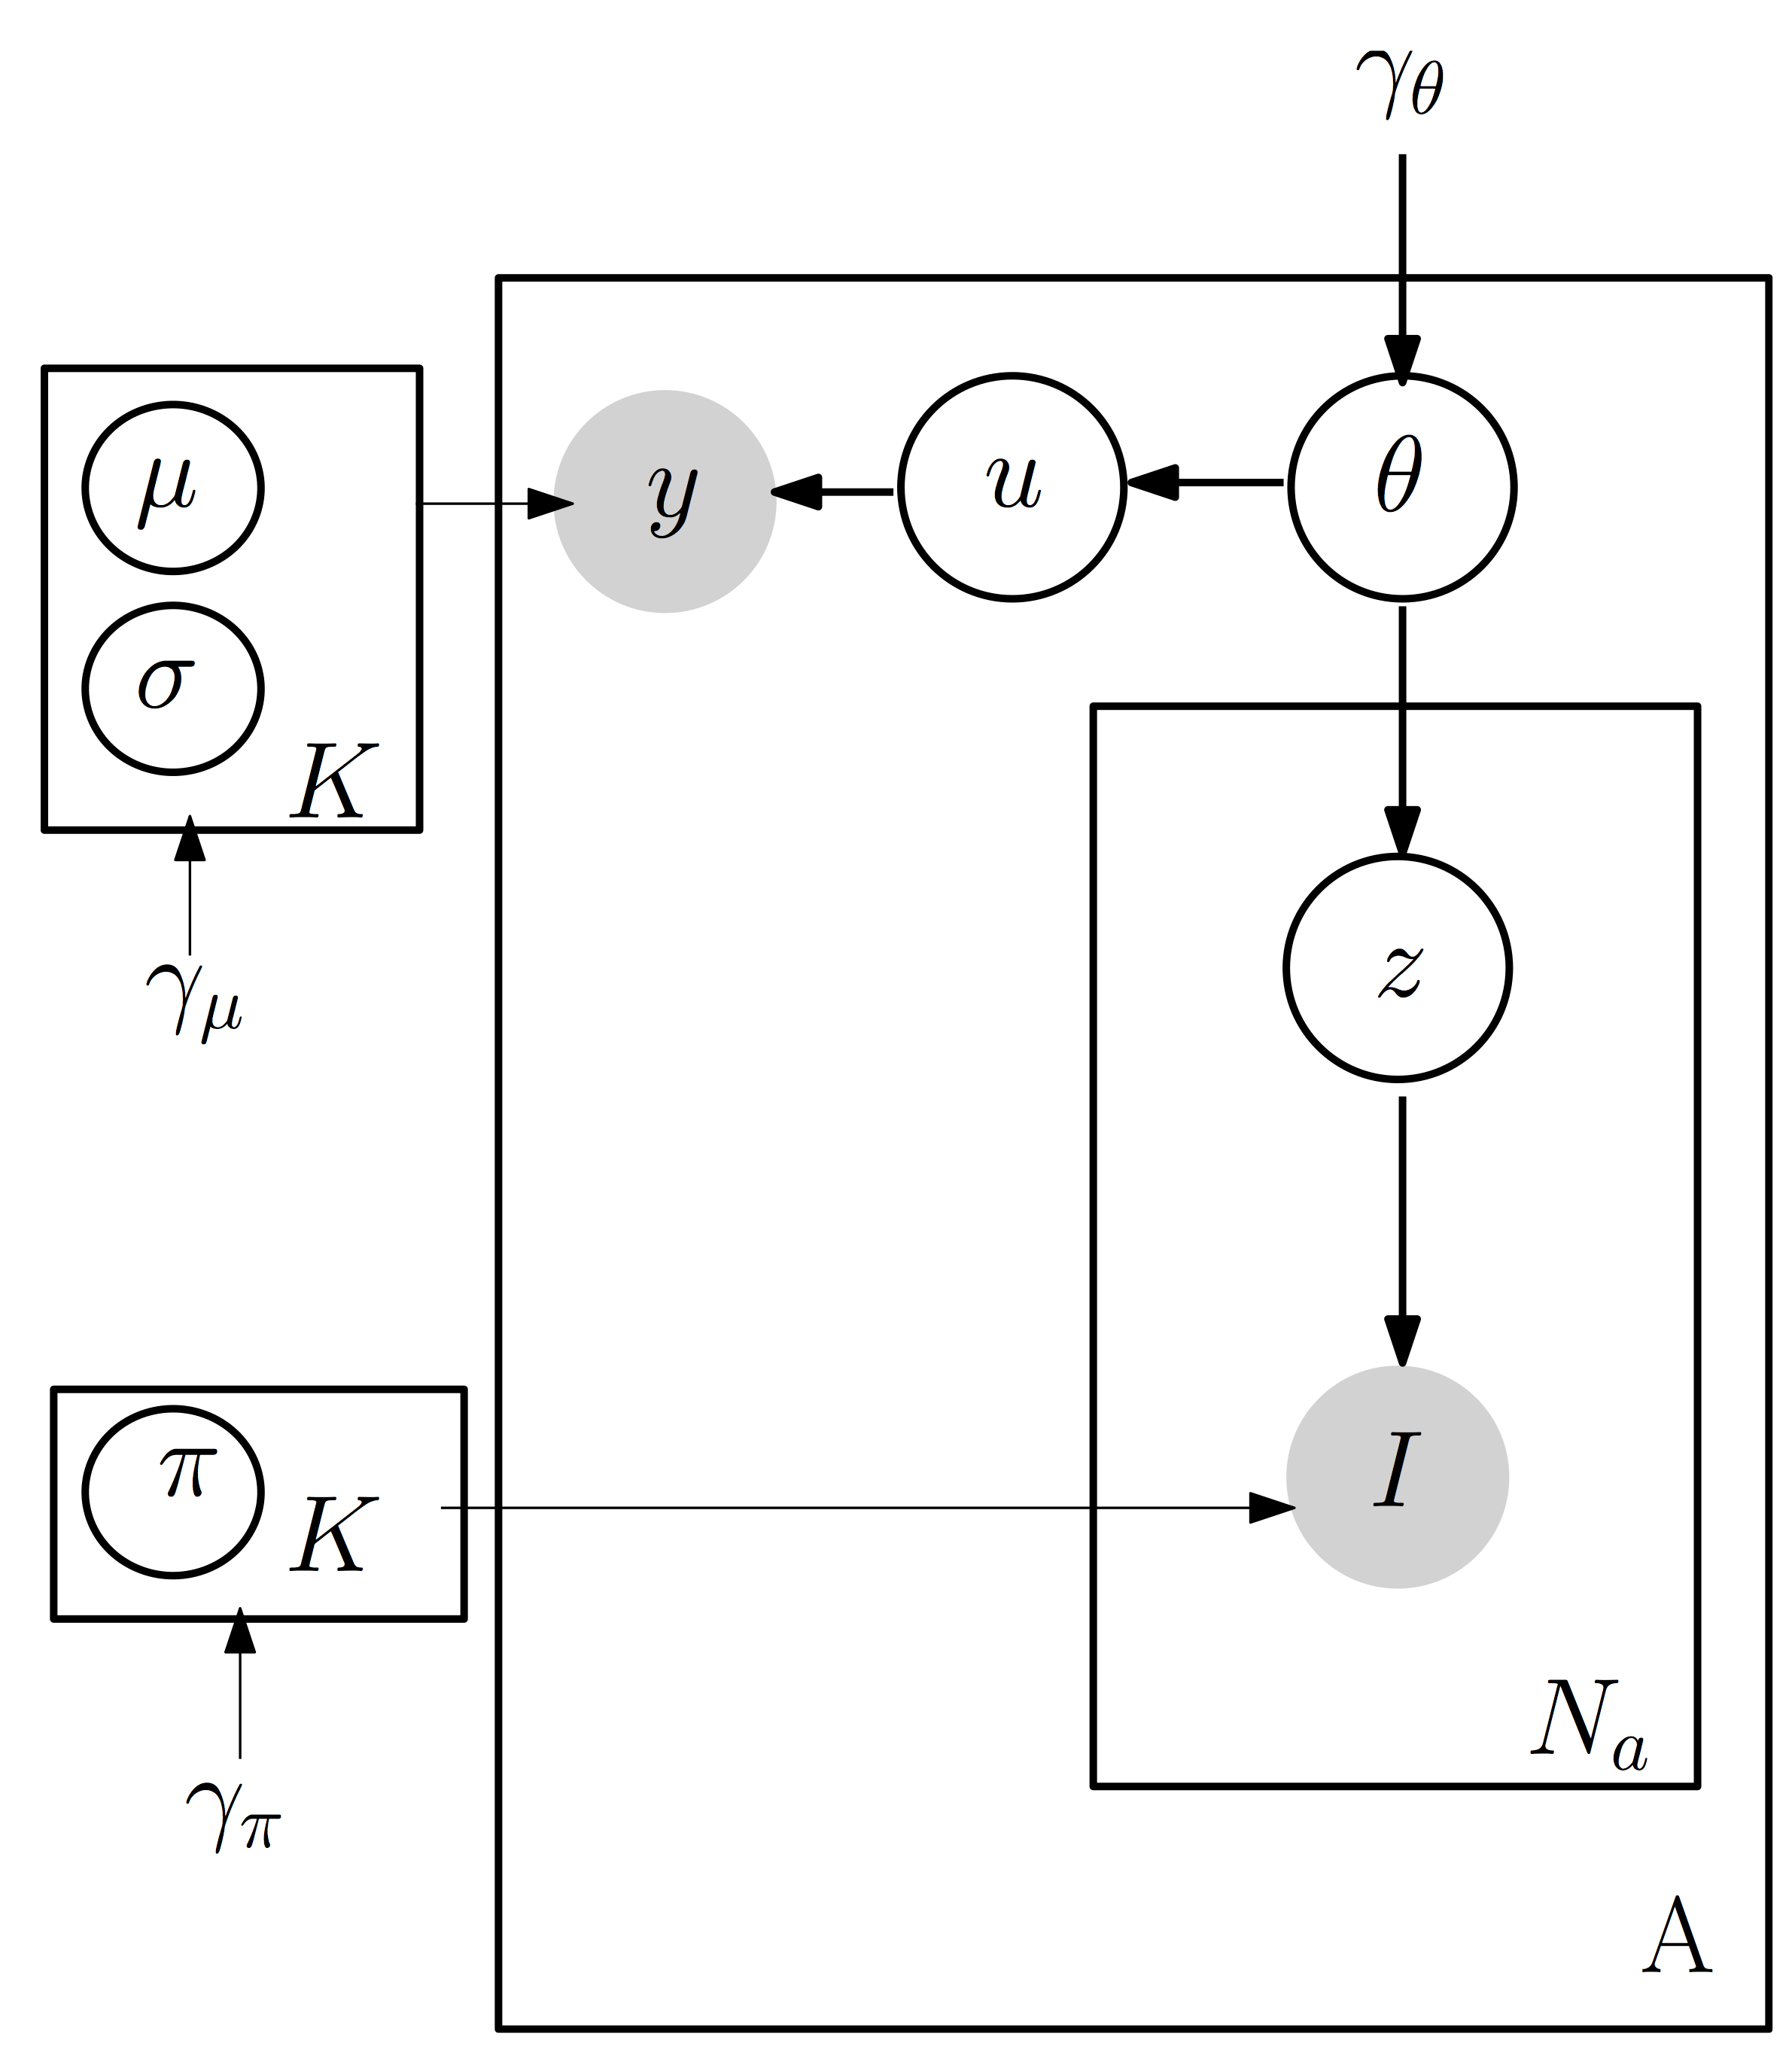
\includegraphics[width=0.6\linewidth]{personaModel}
     \caption{Plate notation of Persona-LDA}
     \label{fig:persona-lda}
\end{figure}
%
%
%When the label sparsity is extreme and each of the data point is mapped to only one label, the multilabel classification problem reduces to the multiclass classification setting. In general cases, 
%Multiclass classification algorithms, which for each data point assigns probability scores to each of the classes, can be used for multilabel classification. In this case, a threshold needs to be identified which will be applied to the probability scores provided by the model: for each data point, sort the probabilities in descending order, from the top predict all the classes for which the probabilities sum to the threshold. This method doesn't handle the label correlations. When labels are ordinal and a test data point is active on more than one labels, this approach is positively biased towards predicting multiple labels which are \textit{consecutive}.
%
%\\\\
%\textbf{Extreme Gradient Boosting (XGBoost):}
%This is a scalable tree boosting methods efficiently optimized to handle sparse data and can be easily distributed. It optimizes a regularized convex loss function and supports shrinkage and column subsampling in addition to the traditional row subsampling to reduce overfitting. It uses approximate algorithm (similar to that in "Parallel boosted regression trees for web search ranking") for split finding instead of using the computationally expensive exact greedy algorithm which enumerates over all possible splits for continuous features. A theoretically guaranteed weighted quantile sketching approach has been proposed to initialize the candidate split points which are then aggregated to find a suitable split. XGBoost is widely used in Machine Learning based industry applications as well as competitions (e.g., Kaggle).
%
\subsection{Algorithms exploiting the label correlation}
\textbf{Power-Set}\\
On the other extreme of binary relevance, Power-Set treats each label subset to be a class and learns a multiclass classifier. If the original label set has L labels, the number of classes will be $2^L$ in worst case. 
This approach is simple, makes coherent predictions and incorporates label dependencies. However it can never predict the label subsets that are not seen in training data. Also, some of the label subsets (or classes) may face scarcity in training data to learn something useful about that class. When the number of label subsets is large, this method is infeasible due to high computational complexity. 

\textbf{Classifier Chains}\\
Classifier Chains (CC) \cite{read2009classifier} is a reduction method which reduces the multi-label problem into $L$ binary classification problems. Unlike binary relevance, it models label correlations in its framework. It uses the chain rule to decompose $p(\textbf{y}\mid\textbf{x})$ into $p(y_1\mid\textbf{x}) \cdot p(y_2\mid \textbf{x},y_1) \cdot p(y_3\mid \textbf{x},y_1,y_2) \cdots p(y_L\mid \textbf{x},y_1,\cdots ,y_{L-1})$ and builds a binary classifier for each of the product term. To classify the labels it decides label $y_l$ by estimating $p(y_l\mid \textbf{x},y_1,\cdots ,y_{l-1})$ and uses $y_l$ as a feature to decide label $y_{l+1}$. As the quality of predictions heavily depend upon the chain order, \cite{read2009classifier} also proposed an ensemble of CCs called Ensemble Classifier Chains (ECC). ECC trains multiple CCs each exposed to a random subset of the data and with random chain order. Then it ensembles the predictions either in individual label wise (ECC-label) or in the level of label subsets (ECC-subset). Recently \cite{liu2015optimality} proposed a dynamic programming approach to predict the chain order optimally but with higher computational complexity. As the predicted subset by standard CC can be faraway from the joint mode, Probabilistic classifier chains (PCC) has been introduced to use more intelligent searching schemes instead of the greedy scheme including $\epsilon$-approximate search \cite{dembczynski2011joint}, Beam search \cite{kumar2012learning}, etc.
%
\\\\
\textbf{Conditional Bernoulli Mixtures (CBM)}
\\
CBM \cite{li2016conditional} models the label correlation by learning a mixture model where each component is modeled as several conditional Bernoulli distributions and choice of the components is modeled as one multinomial distribution.
More specifically the mixture model is presented as: 
\begin{equation}
p(\mathbf{y}\mid\mathbf{x}) = \mathlarger{\sum}\limits_{k=1}^{K} \pi(z=k \mid \mathbf{x};\boldsymbol{\alpha}) \prod_{l=1}^{L} b(y_l \mid \mathbf{x};\boldsymbol{\beta}_l^k)
\end{equation}
where $\pi$ represents the conditional mixture membership distribution with parameter $\boldsymbol{\alpha}$. $b$ represents the conditional binary label distribution with parameter $\boldsymbol{\beta}_l^k$ and $K$ is the number of components. 
Intuitively CBM partitions the data point space in to multiple components and inside each component the labels are assumed to be conditionally independent (conditioned on features). 
The model follows a generative process where for each data point the label set is generated by choosing 1 out of $K$ components from the mixture distribution $\pi$ (say the chosen is $k$) and choosing a label subset from the component specific distribution over label subsets, i.e., $\boldsymbol{\beta}_{\cdot}^{k}$. The mixture distribution $\pi(z \mid \mathbf{x};\boldsymbol{\alpha})$ can be instantiated by a multiclass classifier with parameters $\boldsymbol{\alpha}$. Each local binary label predictor $b(y_l \mid \mathbf{x};\boldsymbol{\beta}_l^k)$ estimates the probability of assigning label $l$ to data point $\mathbf{x}$ in component $k$ which can be instantiated by a binary classifier with parameter $\boldsymbol{\beta}_l^k$. That indicates CBM as a reduction approach that can re-use many well developed algorithms in the literature of binary and multiclass classification.

If CBM has only one component, i.e.,$K=1$, the term $\pi(z \mid \mathbf{x};\boldsymbol{\alpha})$ vanishes and the model reduces to binary relevance. On the other extreme if $K$ is high enough to contain all the possible label sets, than the model reduces to Power-Set. So the number of components with the expressiveness of the components span a spectrum of models between binary relevance and Power-Set.

CBM can be trained by using EM to minimize an upper bound of the negative log-likelihood. The updates for $\boldsymbol{\alpha}$ reduces to a multiclass classification task and the updates for $\boldsymbol{\beta}$ reduces to $K \times L$ binary classification tasks. Any classification algorithm providing soft probability scores over the classes can be used for these tasks, e.g., logistic regression, gradient boosted decision trees, etc.
To make predictions it is required to find the most probable label subset $\mathbf{y^{*}} = argmax_{\mathbf{y}}   \hspace{2mm} p(\mathbf{y} \mid \mathbf{x})$. Computing this exactly is intractable due to $2^L$ possible label subsets. The authors proposed a sampling based approach which solves this optimization problem approximately. They also discussed a dynamic programming based approach to solve the problem exactly but with higher running time. 
%\\\\
%\textbf{Handling Missing labels using Matrix completion techniques}
%
%
%It works with three kinds of distributions: for each household, a multinomial distribution over personas and for each persona, a multinomial distribution over items and a gaussian distribution over age. 
%[To be included in experiments Discussion: ] Note that we don't compare our proposed approach with Persona-model[?] due to its high running time.
%
%\section{Related work}
\section{Experiments}
\label{sec:experiments}
In this section we compare various multilabel algorithms in their ability to predict the household composition. We discuss the effect of label noise and feature noise in the training data on the performance. We also provide some interpretable explanations for the predictions through the lens of ASINs with an analysis on prediction error.  Formally we conduct three types of experiments. (1) Jointly discovering age and gender composition. (2) Investigating the effect of feature noise and label noise in the training data. (3) Explaining the model through interpretable features. 
%
%\begin{table*}[]
%\centering
%\caption{My caption}
%\label{my-label}
%\begin{tabular}{|c|c|c|c|c|c|c|}
%\hline
%\textbf{}                   & \textbf{}                                                             & \textbf{Fashion Survey} & \multicolumn{2}{c|}{\textbf{Kindle Household}}                                                                                      & \multicolumn{2}{c|}{\textbf{Own Survey}}                                                                                            \\ \hline
%\textbf{Algorithm}          & \textbf{\begin{tabular}[c]{@{}c@{}}Experimental\\ Setup\end{tabular}} & \textbf{Accuracy}       & \textbf{\begin{tabular}[c]{@{}c@{}}Macro \\ Jaccard\end{tabular}} & \textbf{\begin{tabular}[c]{@{}c@{}}Exact \\ Match\end{tabular}} & \textbf{\begin{tabular}[c]{@{}c@{}}Macro \\ Jaccard\end{tabular}} & \textbf{\begin{tabular}[c]{@{}c@{}}Exact \\ Match\end{tabular}} \\ \hline
%%Multiclass XGBoost          & Setup A                                                               & 42.38                   & 41.46                                                             & 41.05                                                           & 52.1                                                              & 44.6                                                            \\ \hline
%Multilabel XGBoost          & Setup D                                                               &43.3                       & 35.4                                                                & 11.4                                                               &38.7                                                                 &9.6                                                               \\ \hline
%CBM                         & Setup C                                                               & ?                       & 32.3                                                              & 28.8                                                            & 55.32                                                             & 46.75                                                           \\ \hline
%Multiclass XGBoost          & Setup D                                                               & 45.22                   & 43.63                                                             & 43.2                                                               & 56.8                                                                 & 48.3                                                               \\ \hline
%LEML          & Setup D                                                               & ?                   & ?                                                             & ?                                                               & ?                                                                 & ?                                                               \\ \hline
%PfastreXML          & Setup D                                                               & ?                   & ?                                                             & ?                                                               & ?                                                                 & ?                                                               \\ \hline
%GBDT-sparse         & Setup D                                                               & ?                   & ?                                                             & ?                                                               & ?                                                                 & ?                                                               \\ \hline
%GenEML         & Setup D                                                               & ?                   & ?                                                             & ?                                                               & ?                                                                 & ?                                                               \\ \hline
%
%%Multiclass Pairwise XGBoost & Setup D                                                               & 45.88                   & 43.17                                                             & 42.74                                                           & ?                                                                 & ?                                                               \\ \hline
%%LSTM                        & Setup E                                                               & 41.06                   & 38.17                                                             & ?                                                               & ?                                                                 & ?                                                               \\ \hline
%%DNN + XGBoost               & Setup F                                                               & 46.85                   & 44.49                                                             & ?                                                               & ?                                                                 & ?                                                               \\ \hline
%%(LSTM+DNN) + XGBoost        & Setup G                                                               & 47.98                   & 45.24                                                             & ?                                                               & ?                                                                 & ?                                                               \\ \hline
%\end{tabular}
%\end{table*}

\textbf{Datasets}\\
%We use the following four datasets in our experiments.\\
\textit{Experian:} 
Amazon obtains customer demographic information from Experian, a third party organization, and matches the data with its 
%Experian is an external organization which provides customer demographic information to Amazon. Amazon matches the Experian data with its 
own customer information based on various criteria such as full name, billing/shipping address, zip code, etc. The resulted data comes with 180MM customers covering around 54\% of Amazon US accounts. A comparison with more accurate survey data conducted by Amazon Fashion team indicates the account holder age labels of Experian to be 63\% accurate.

\textit{Kindle household: } Kindle household data, collected by the Household team of Kindle, claims to contain the household composition for around 13MM households in US. Essentially it contains the mapping of accounts that belong to the same household. As per the data, only 220K households out of 13MM have more than one member, which is 1.7\% (against 64\% as per US census) \footnote{This indicates that Kindle household is partially labelled}. In the sequel, we refer to this subset of 220K as \textit{K-Multi-household} data.

%\textit{Fashion Survey:} Amazon Fashion team has conducted a survey with 10365 customers. It records the account holder age band and is suitable to evaluate a model for account holder age prediction. 
%
\textit{ICT:} This data has been collected from the Amazon retail internal consumer tracker survey and consists of 22900 customers. It records the account holder age band with gender. It is suitable to be used  to evaluate a model for account holder age or gender prediction. 

\textit{MLBLR-survey:} As we couldn't find any existing data on the complete household composition, we conducted a survey by sending requests to a small group of Amazon employees. For each account we recorded the age and gender composition of both adult and child members of the household. This dataset contains 1170 households.

Figure ~\ref{fig:datasets} demonstrates the age group proportions in each dataset. The distribution of Kindle household and Experian are very similar. ICT and the MLBLR-survey are very different from each other; while ICT is more biased towards older population, MLBLR-survey is more biased towards younger population.
%
%
\begin{figure}
\setlength{\belowcaptionskip}{-10pt}
  \centering
    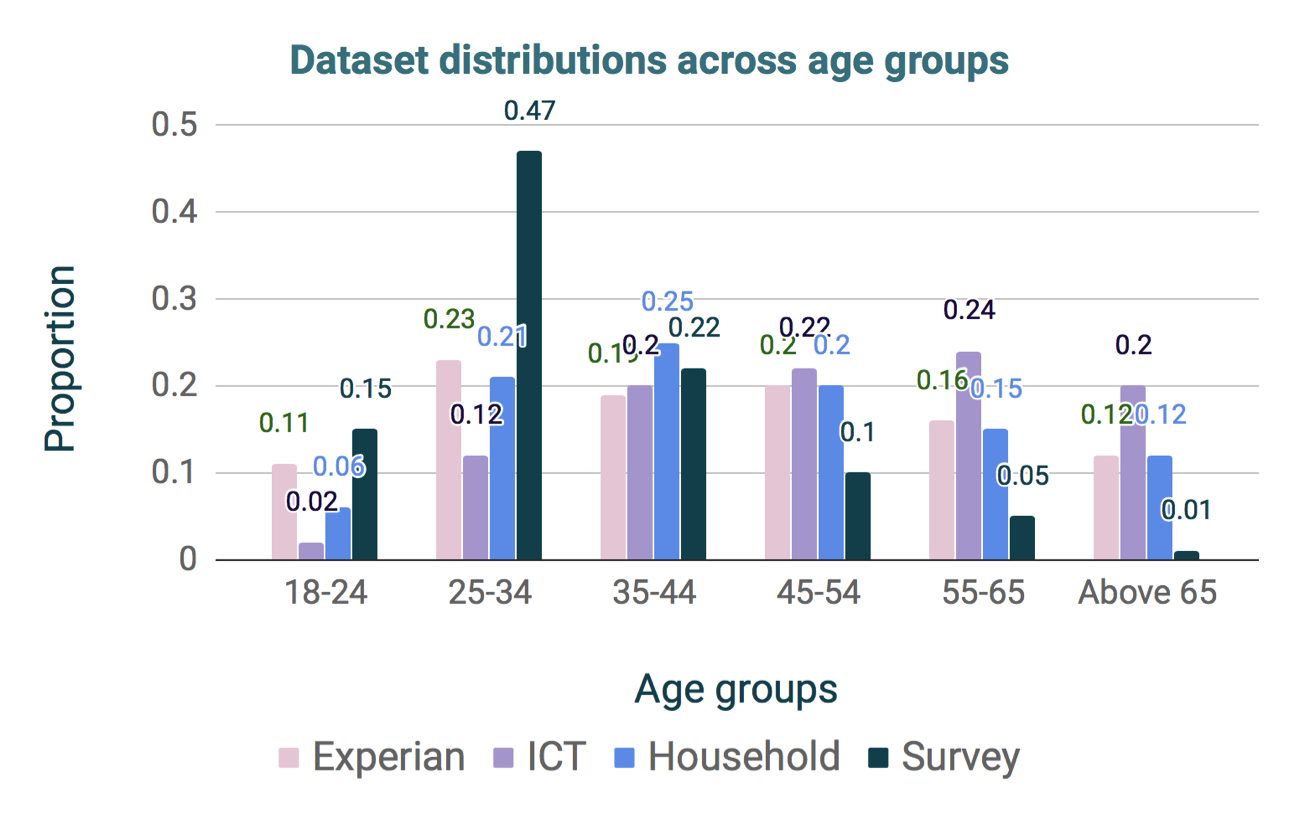
\includegraphics[width=0.99\linewidth]{datasetDistributions3.png}
  \caption{Distributions of various datasets. }
  \label{fig:datasets}
\end{figure}
%

\textbf{Feature Engineering}\\
For each customer account, we have two sets of features: a set of purchase based features and a set of static features. Purchase based features include titles, brand names, brand IDs and interest mapping of ASINs purchased by the customer \cite{sohoney2016interest}, RFM (recency, frequency and monetary) values for each GL and customer subscriptions. 
For titles and brand names, we tokenize them to get tuples and perform TFIDF (section 6.2.2 of \cite{christopher2008introduction} on the tuples. We further perform a symmetric uncertainty based feature selection optimizing normalized mutual information on the tuples to identify tuples that are predictive of age. We used brand IDs of the top 200 most purchased ASINs and the interest mappings membership as described in \cite{sohoney2016interest}. 
To get the top predictive subscriptions, we performed feature selection on the subscriptions over 1 year period. For all the purchase based features, we use past 5-year purchases.
%
The set of static features include customer account level features such as customers' first and last name, billing zip code, email domain, etc. 
%We use 2-grams of the first and last name. 
For all the experiments we use around 11.3K purchase based features and 5K account level static features.
%
%\begin{figure*}
%  \centering
%  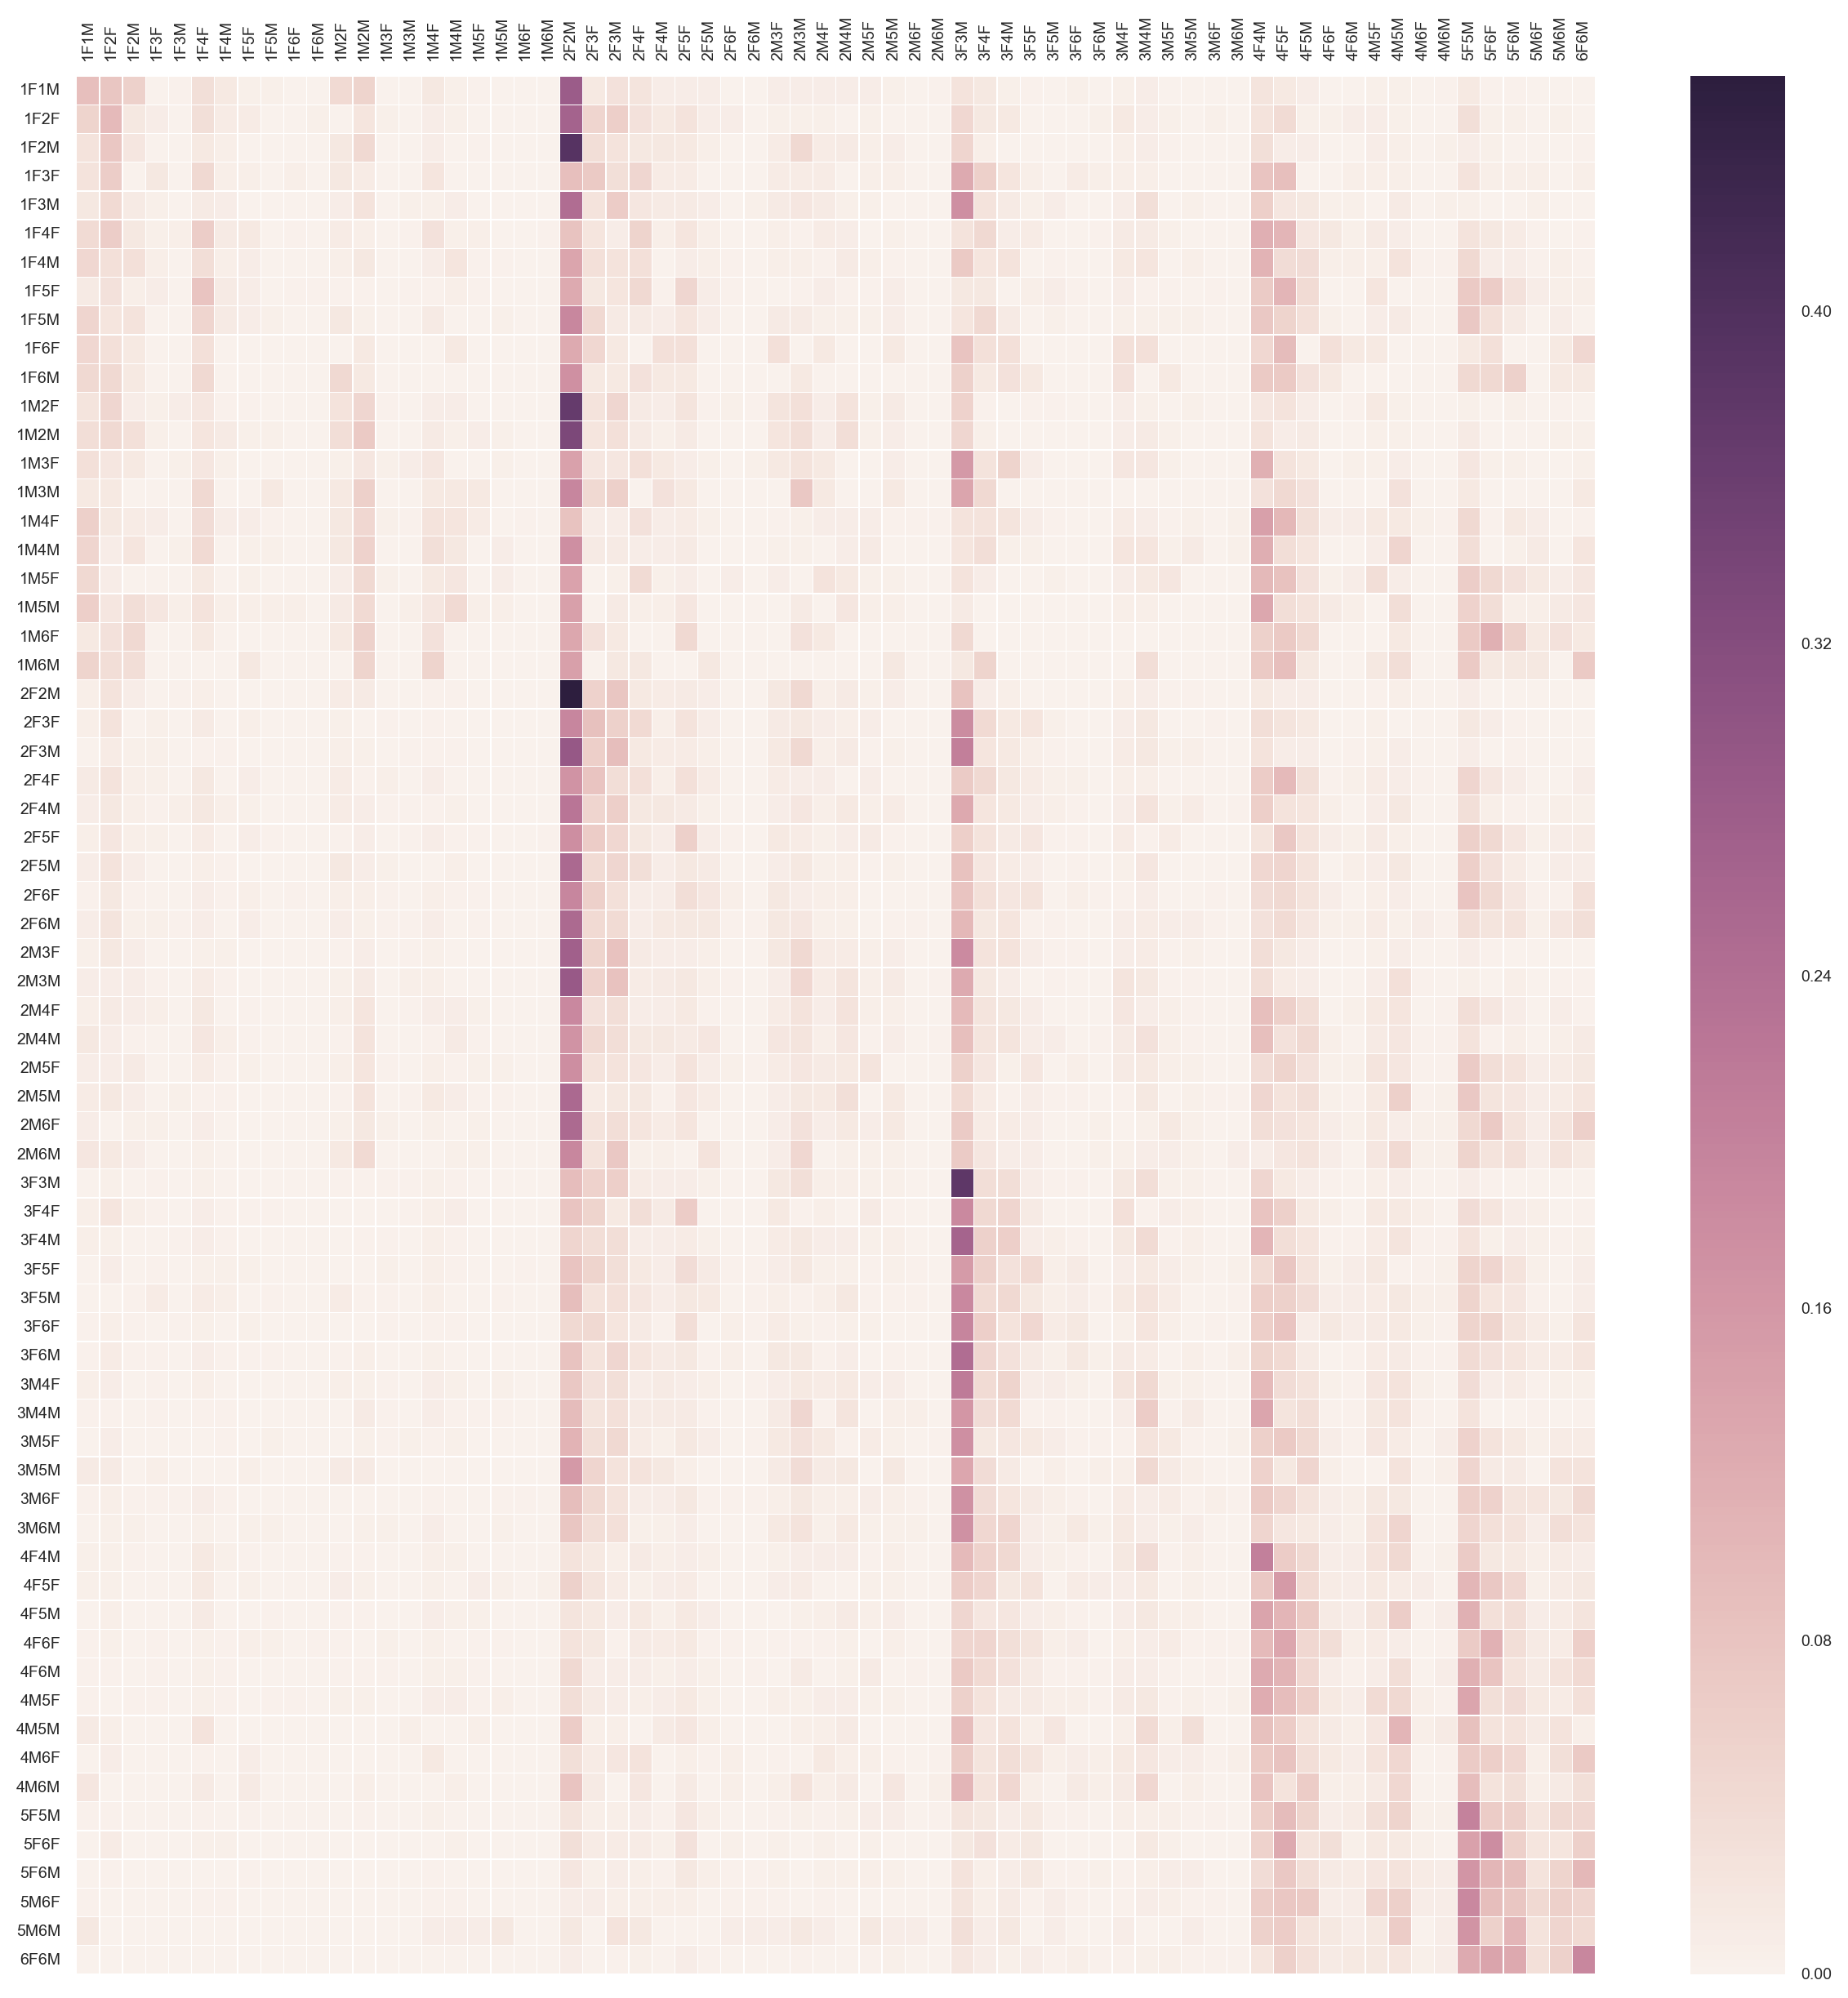
\includegraphics[width=.45\linewidth]{Plots/confusionHeatmap_br.png}
%  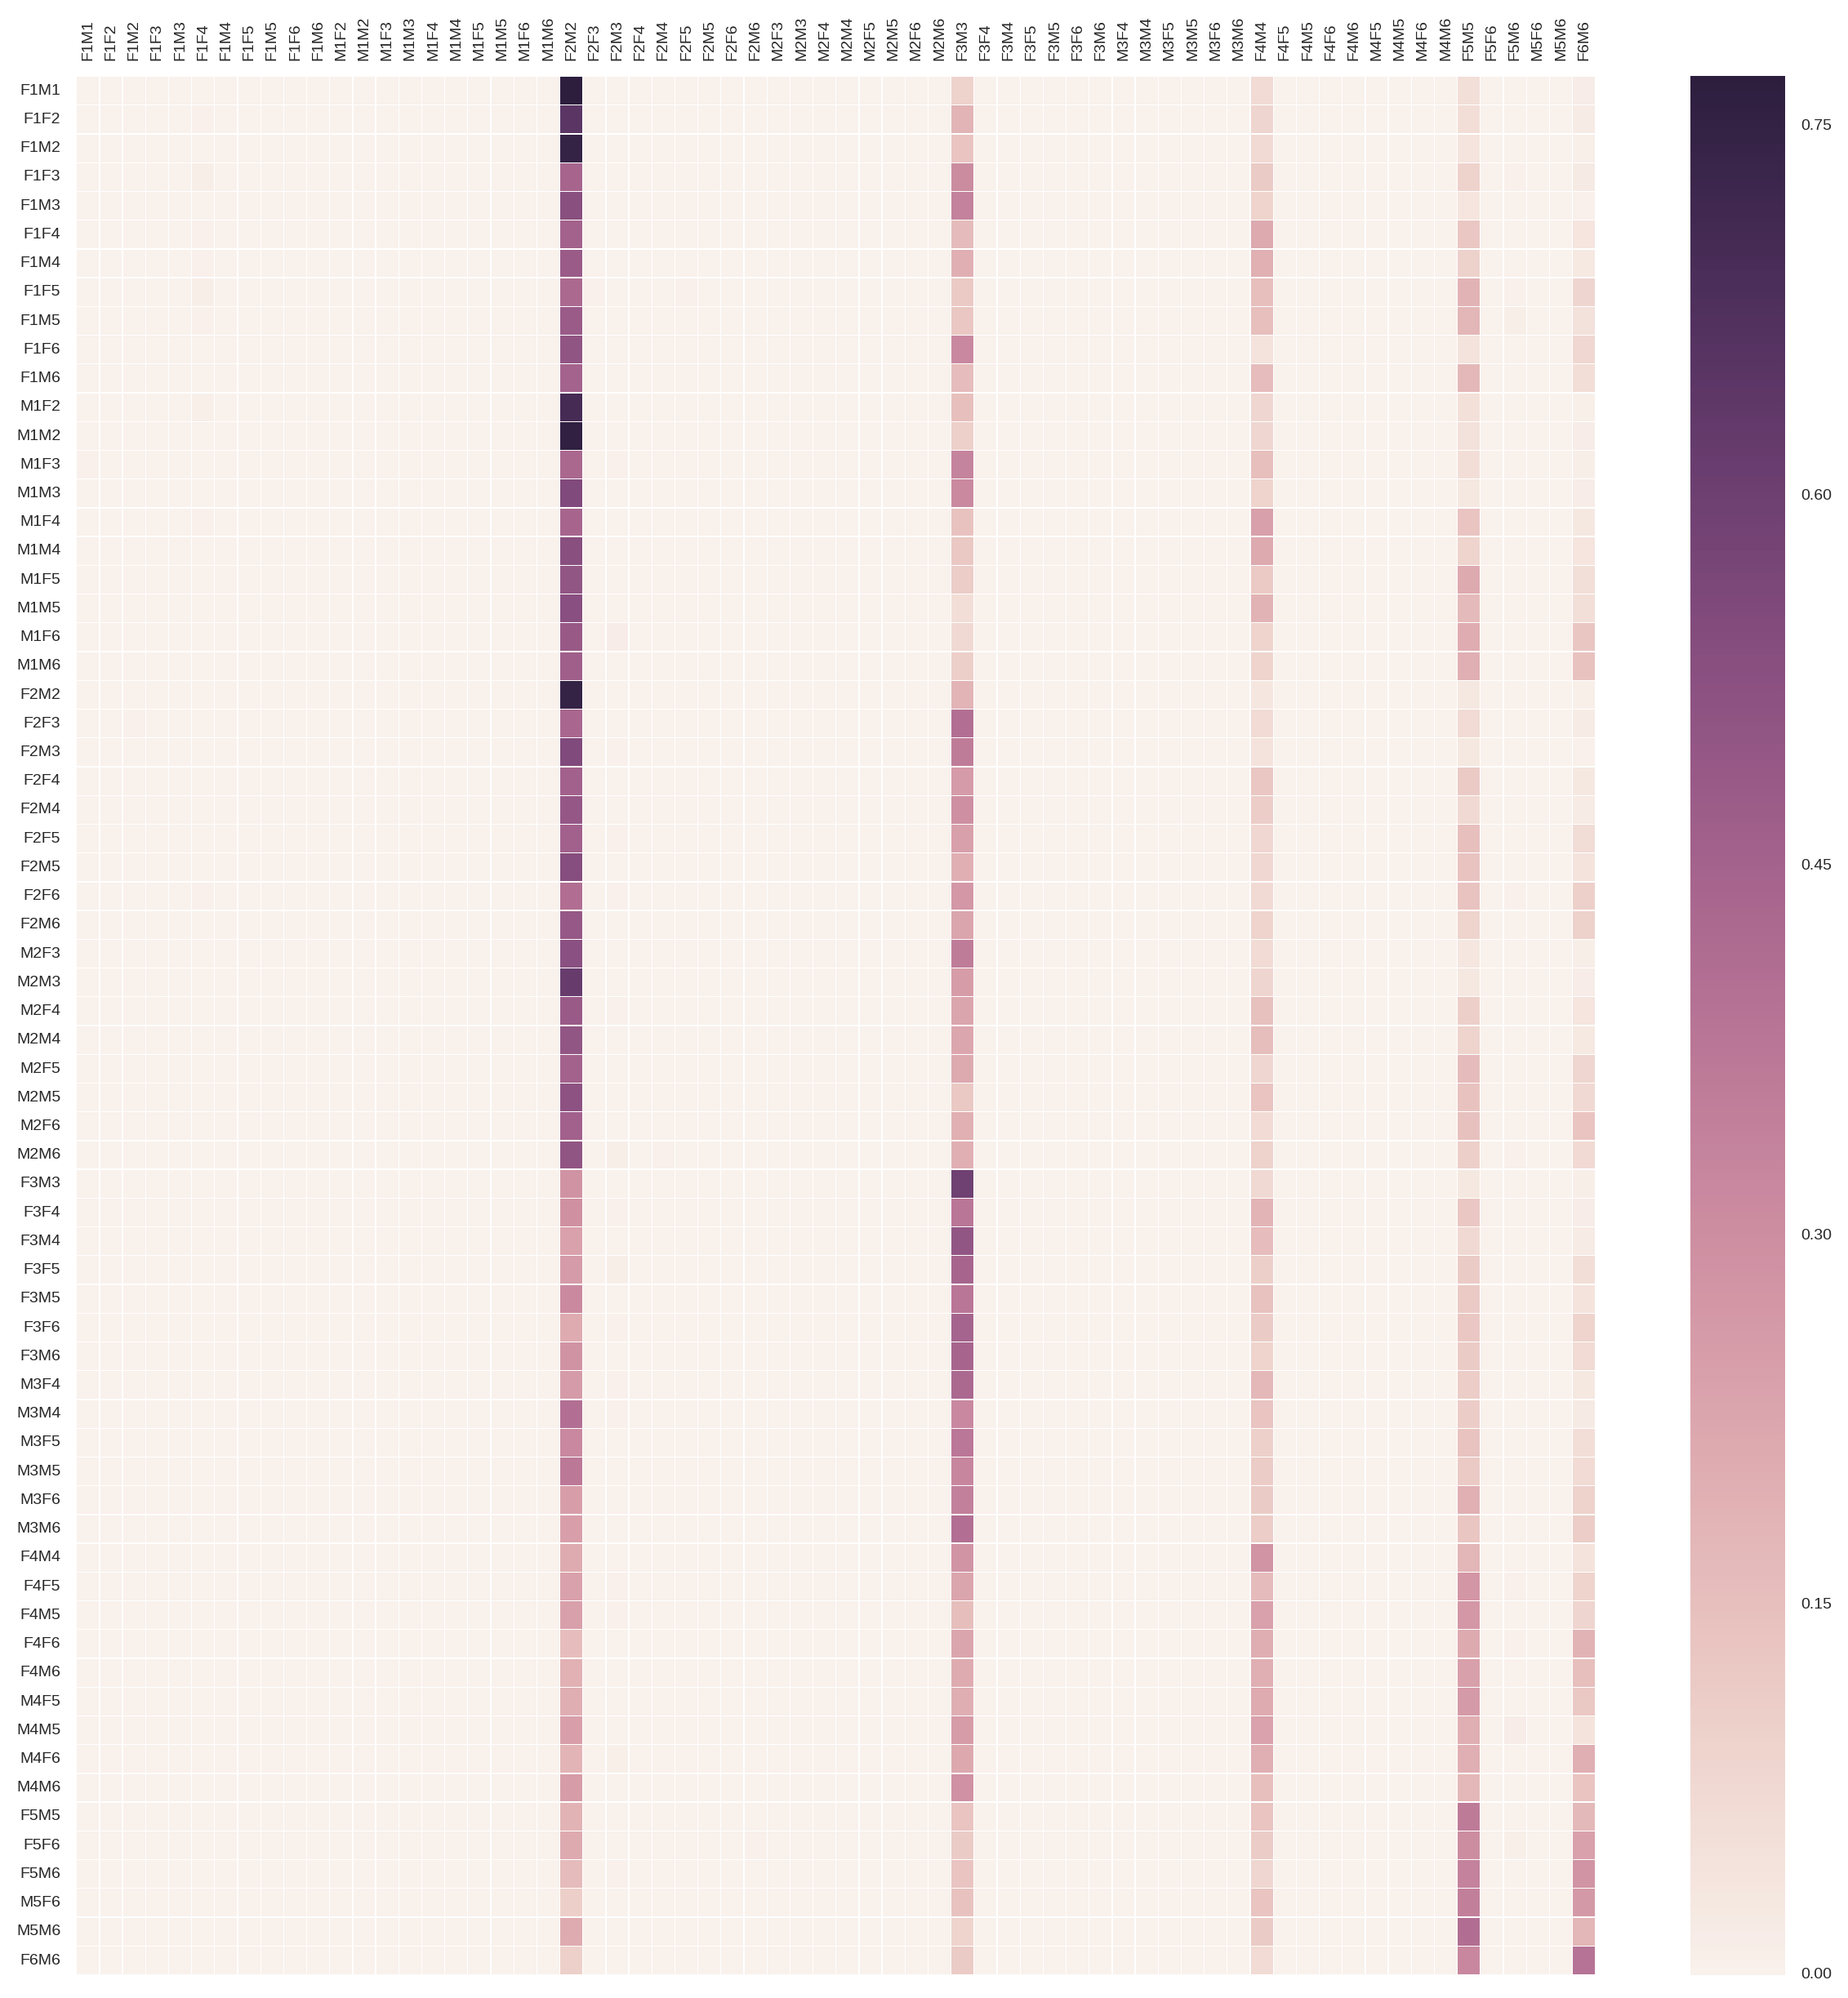
\includegraphics[width=.45\linewidth]{Plots/confusionHeatmap_cbm.png}
%  \caption{ Confusion matrix generated from ground truth and predictions by binary relevance (left) and CBM (right).}
%  \label{fig:confmat-br-cbm}
%\end{figure*}
%
\begin{table*}[]
\small
\setlength{\belowcaptionskip}{-10pt}
\centering
\begin{tabular}{|c|c|c|c|c|}
\hline
                                             & \multicolumn{2}{c|}{\textbf{K-Multi-Household}} & \multicolumn{2}{c|}{\textbf{MLBLR Survey}} \\ \hline
\textbf{Algorithm}                           & Macro-Jaccard          & Exact Match          & Macro-Jaccard         & Exact Match        \\ \hline
\textbf{Binary Relevance (BR)}               & 31.24\%                & 3.09\%               & 24.43\%               & 0.00\%             \\ \hline
\textbf{BR-Max-2}                            & 32.58\%                & 16.21\%              & -                     & -                  \\ \hline
\textbf{CBM}                                 & \textbf{33.35}\%                & \textbf{21.87}\%              & \textbf{43.14}\%               & \textbf{28.35}\%            \\ \hline
\textbf{Baseline (Majority)} & 21.72\%                & 12.65\%              & 38.98\%               & 24.68\%            \\ \hline
\end{tabular}
\caption{Performance of various techniques in discovering age and gender composition. }
\label{table:performance-age-gender}
\end{table*}
%
\begin{figure*}
\setlength{\belowcaptionskip}{-10pt}
  \captionsetup{font=small}
  \centering
  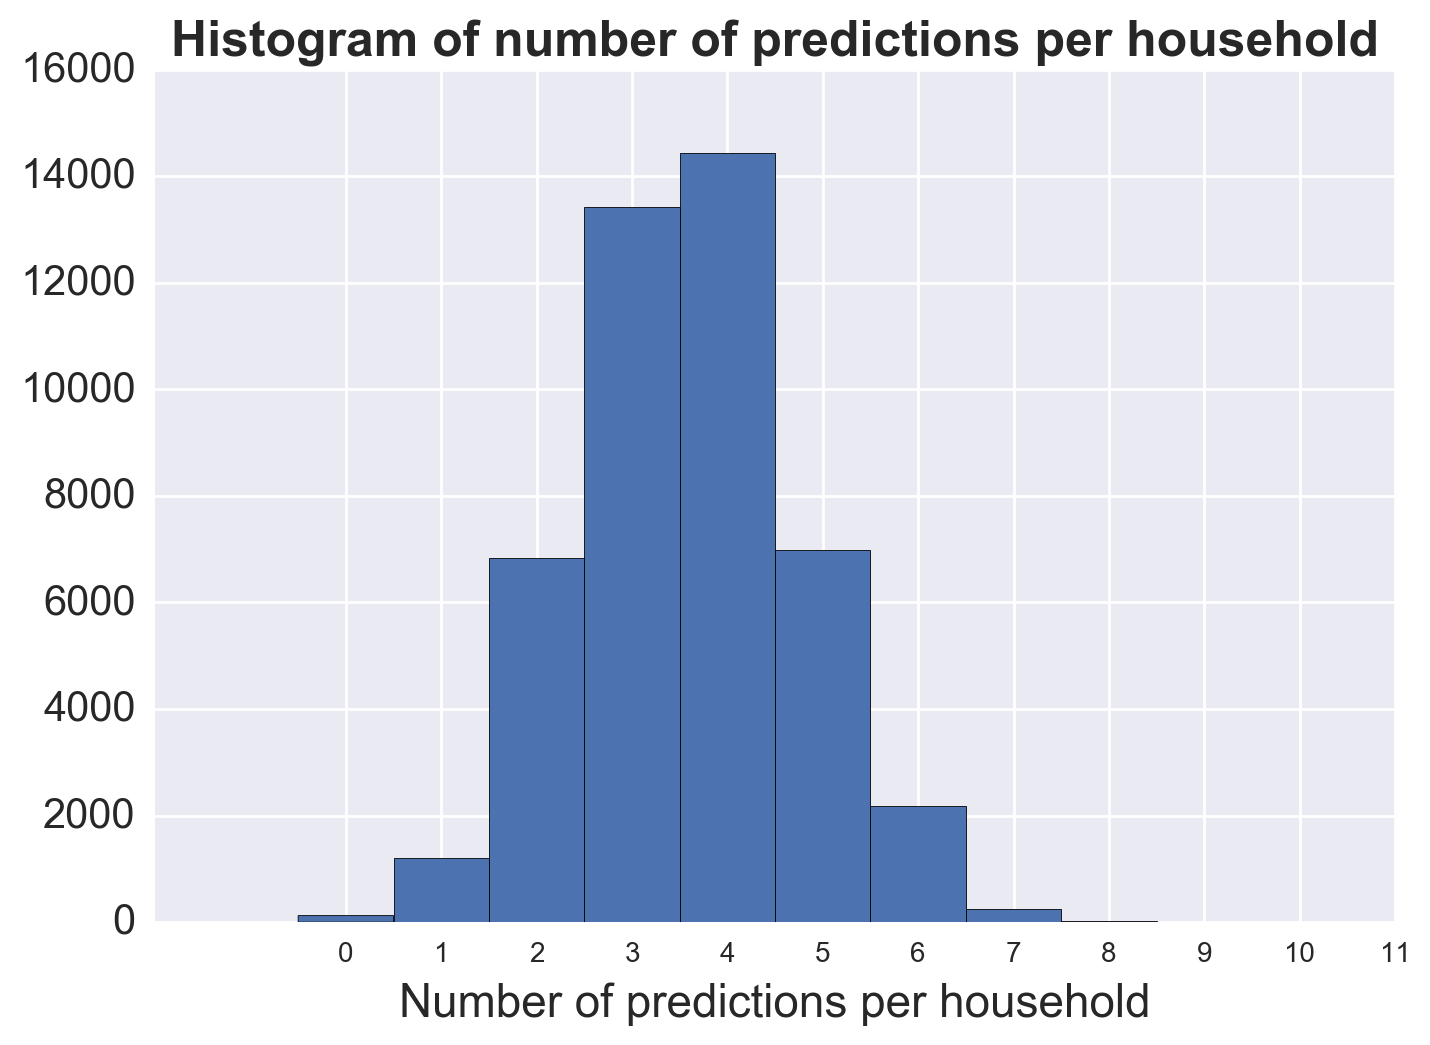
\includegraphics[width=.45\linewidth]{predictionHistogram2.png}
  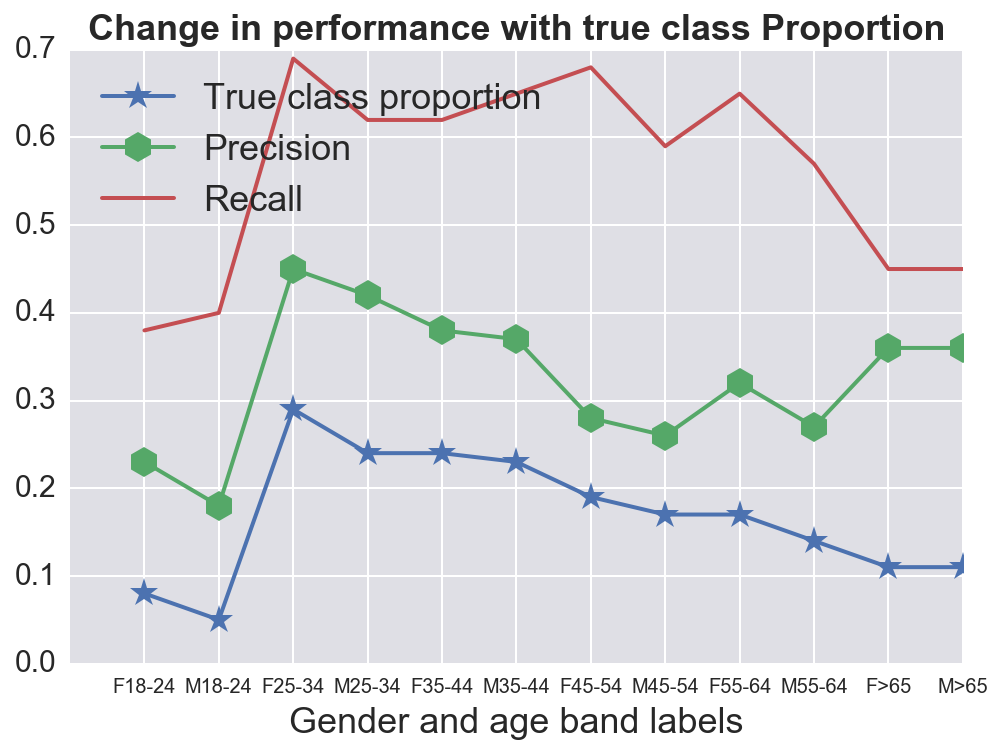
\includegraphics[width=.45\linewidth]{br_allLabels2.png}
  \caption{\textit{Left:} Distribution of number of persons per household predicted by Binary Relevance, \textit{Right}: Label wise precision and recall with increasing threshold.}
  \label{fig:histogram-br}
\end{figure*}

\begin{figure*}
  \captionsetup{font=small}
  \setlength{\belowcaptionskip}{-10pt}
  \centering
  %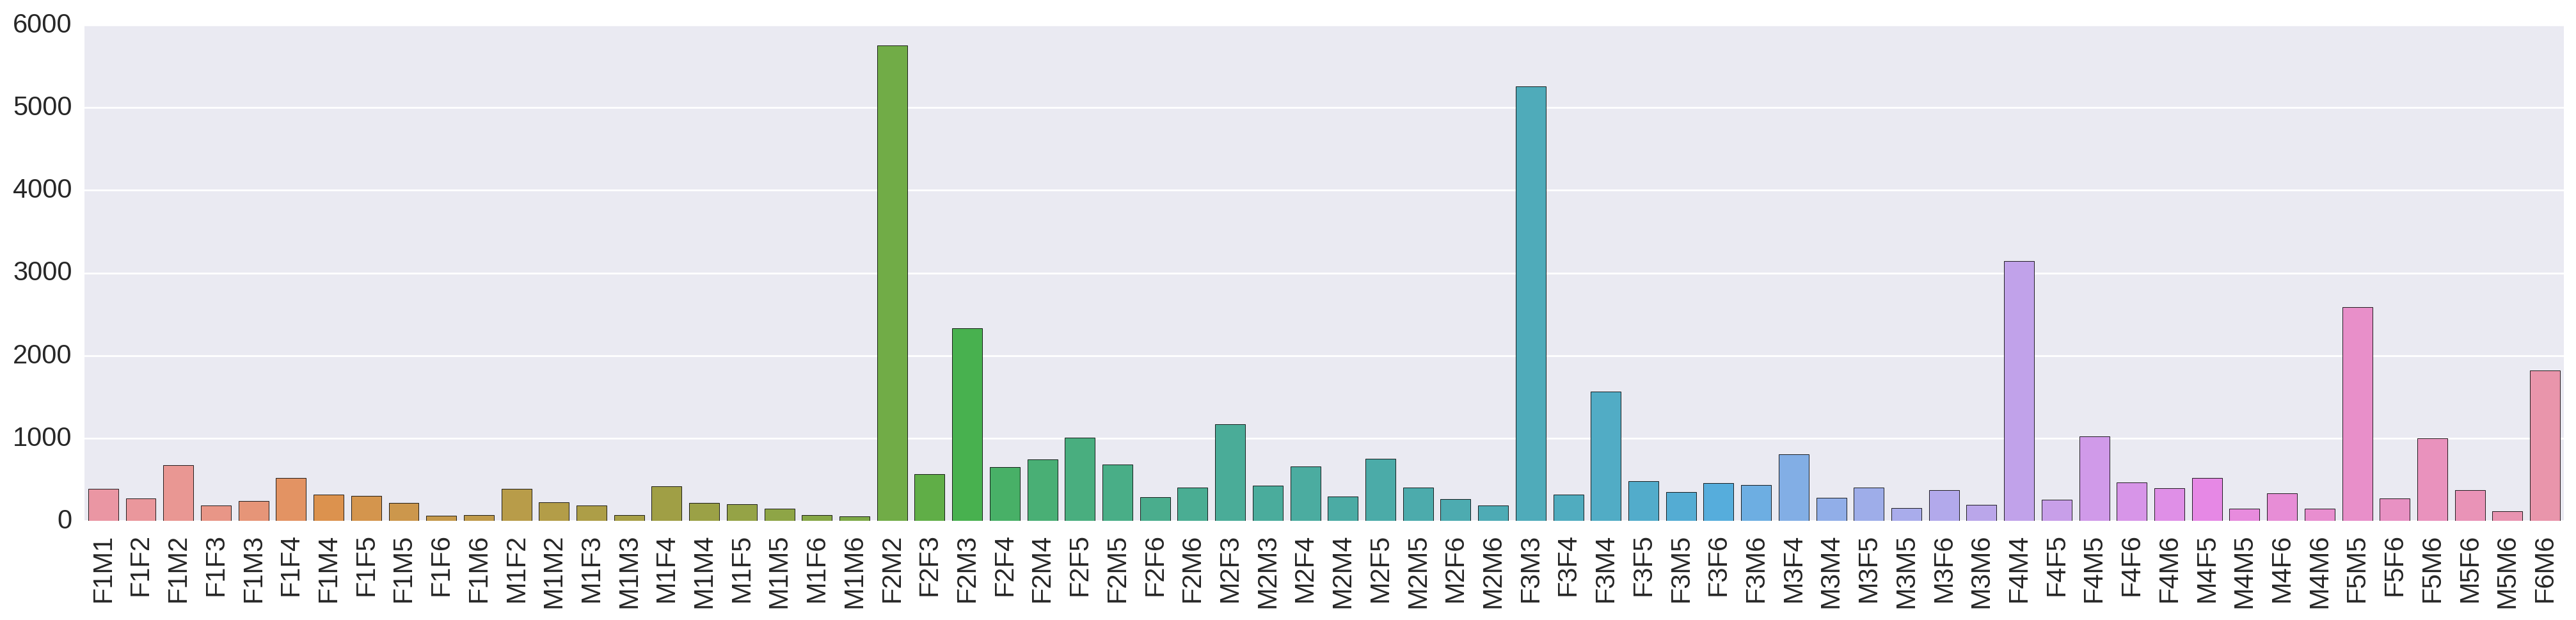
\includegraphics[width=0.48\linewidth]{Plots/gtruth_multihh.png}
  %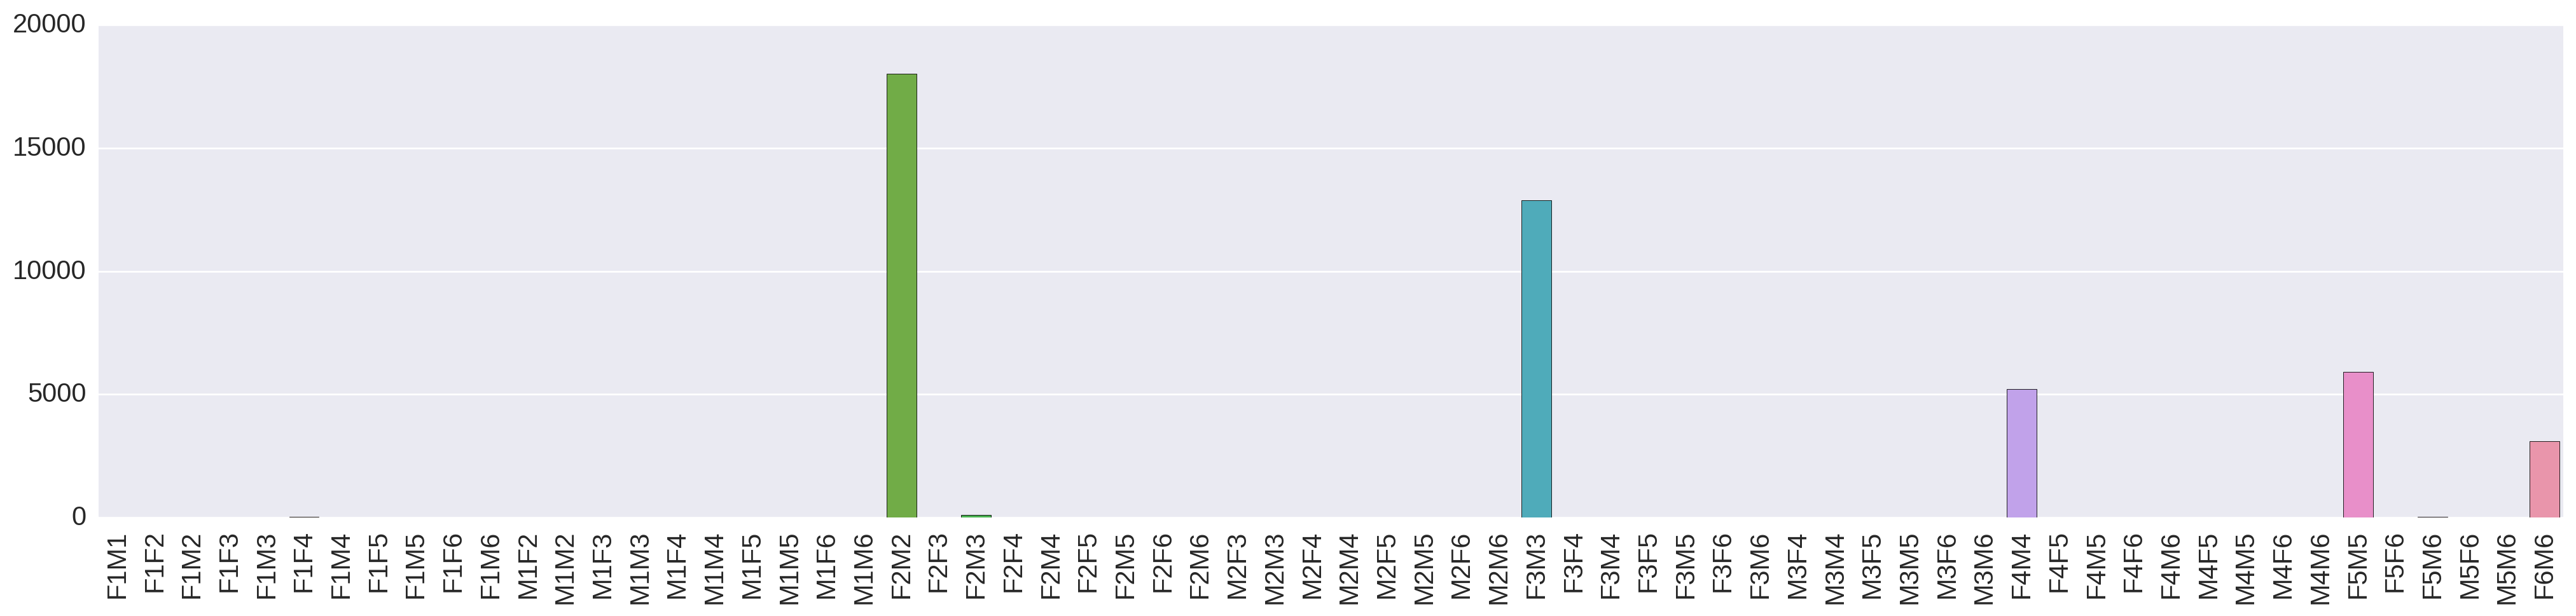
\includegraphics[width=.48\linewidth]{Plots/prediction_multihh_CBM.png}
  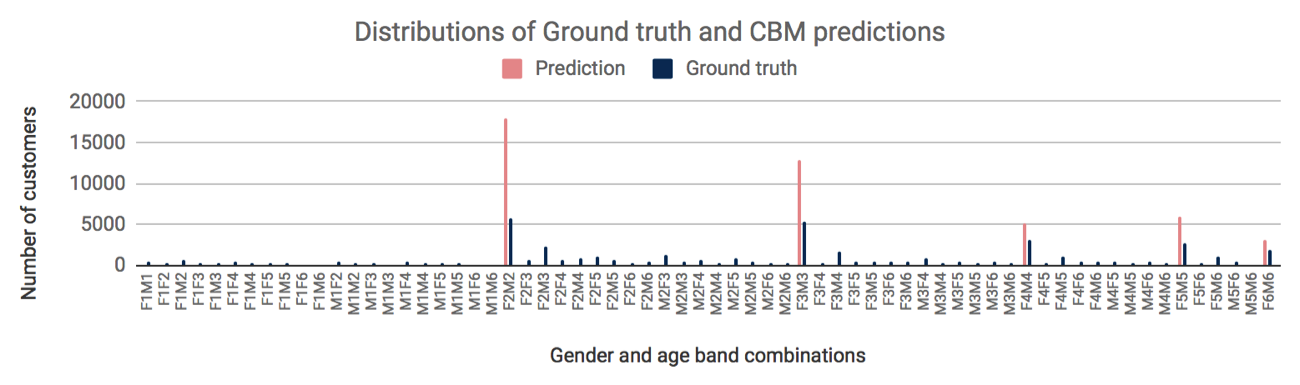
\includegraphics[width=.99\linewidth]{cbmPredictions3.png}
  \caption{ \textit{Histogram of ground truth labels and predictions by CBM}: The labels in X axis are shorthands for households, e.g., F2M3 denotes a household with one female with age 25-34 and one male with age 35-44. 
  %The bars denote the number of accounts in the ground truth and prediction, e.g., 18K accounts are predicted to be in F2M2, while the ground truth had only 6K households. 
  We see that predictions are concentrated on households with 2 members from the same age group with different gender.}
  \label{fig:histogram-cbm}
\end{figure*}
%
%\begin{figure*}
%  \centering
%  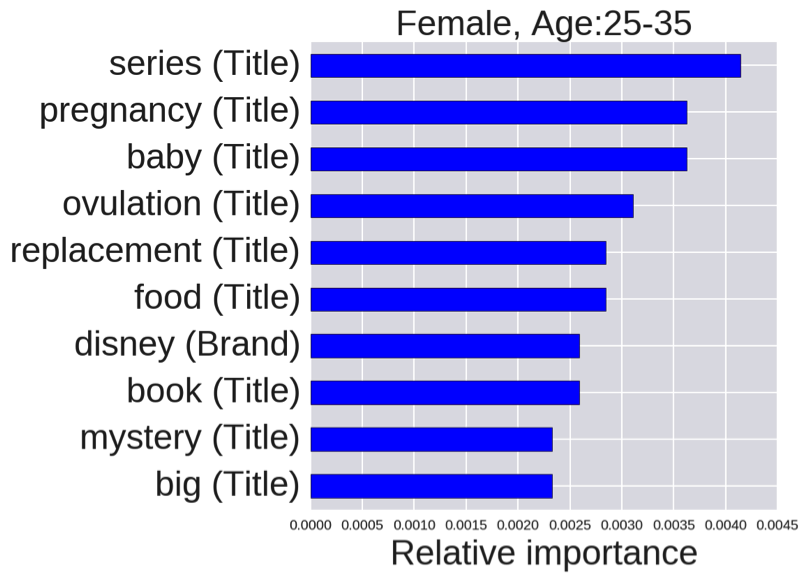
\includegraphics[width=0.4\linewidth]{Plots/topFeatures1.png}
%  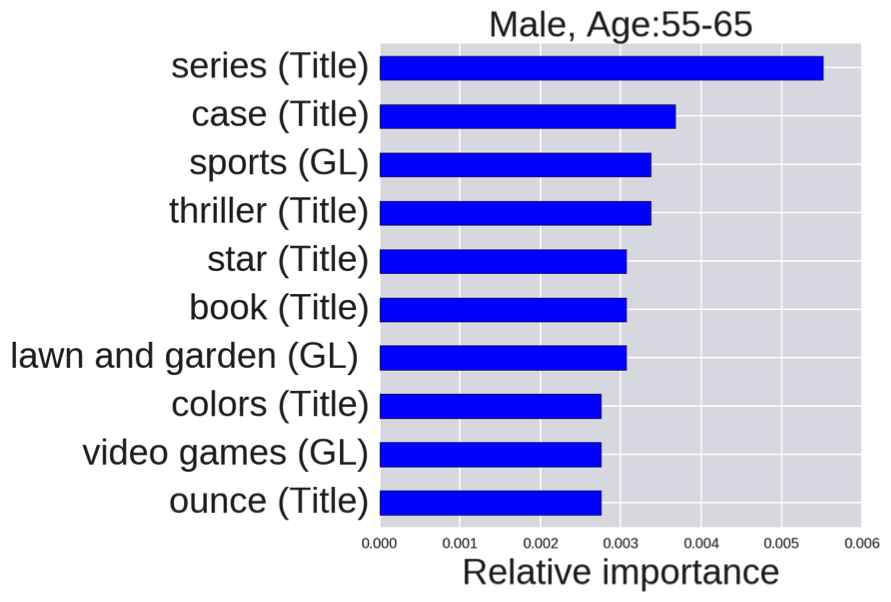
\includegraphics[width=.4\linewidth]{Plots/topFeatures2.png}
%  \caption{Top features learnt by XGBoost with their relative scores.}
%  \label{fig:topfeatures-XGBoost}
%\end{figure*}
%
%
%
%
%
\textbf{Evaluation Metrics}\\
We consider Exact Match and Macro-Jaccard to measure the quality of the predictions. Let $N$ be the number of accounts and for the $i^{th}$ account,  $Y_i$ and $Z_i$ be the set of true labels and predicted labels, respectively. 
\textit{Exact Match} is defined as  $\frac{1}{N} \sum_{i=1}^N \|Y_i = Z_i \|$ , i.e., proportion of households for whom the entire demographic composition was predicted correctly.  This is arguably a stringent metric giving credit only if the predicted label set is exactly equal to the true set of labels. A more appropriate relaxed version is \textit{Macro-Jaccard} accuracy which is defined as $\frac{1}{N}\sum_{i=1}^N \frac{\|Y_i \cap Z_i \|}{\|Y_i \cup Z_i \|}$. This smoothly penalizes both under prediction and over prediction discrepancies. 
We consider \textit{multiclass accuracy} to measure the quality of account holder age prediction.
%
%
\begin{table*}[]
\setlength{\belowcaptionskip}{-10pt}
\small
\centering
\begin{tabular}{|c|c|c|c|c|c|c|}
\hline
\textbf{}                      & \multicolumn{2}{c|}{\textbf{K-Multi-Household}} & \multicolumn{2}{c|}{\textbf{MLBLR Survey}} & \multicolumn{2}{c|}{\textbf{Kindle Household}} \\ \hline
\textbf{Algorithm}             & Macro-Jaccard          & Exact Match          & Macro-Jaccard         & Exact Match        & Macro-Jaccard           & Exact Match          \\ \hline
\textbf{Binary Relevance (BR)} & \textbf{41.83}\%                & 9.48\%               & 38.7\%               & 9.6\%             & 35.40\%                 & 11.40\%              \\ \hline
%\textbf{BR-Max-1}              & 44.41\%                & 21.08\%              & -                     & -                  & -                       & -                    \\ \hline
\textbf{CBM}                   & 39.95\%                & 21.94\%              & 55.32\%               & 46.75\%            & 32.29\%                 & 28.77\%              \\ \hline
\textbf{Multiclass XGBoost}            & 40.31\%                & \textbf{22.82}\%              & \textbf{66.69}\%               & \textbf{58.43}\%            & \textbf{40.43}\%                 & \textbf{40.01}\%              \\ \hline
\textbf{Baseline}              & -                      & -                    & 50.83\%               & 45.24\%            & 24.66\%                 & 24.37\%              \\ \hline
\end{tabular}
\caption{Performance of different techniques in discovering age composition.}
\label{table:performance-age}
\end{table*}
%
%
%
%
%\begin{figure}
%  \centering
%  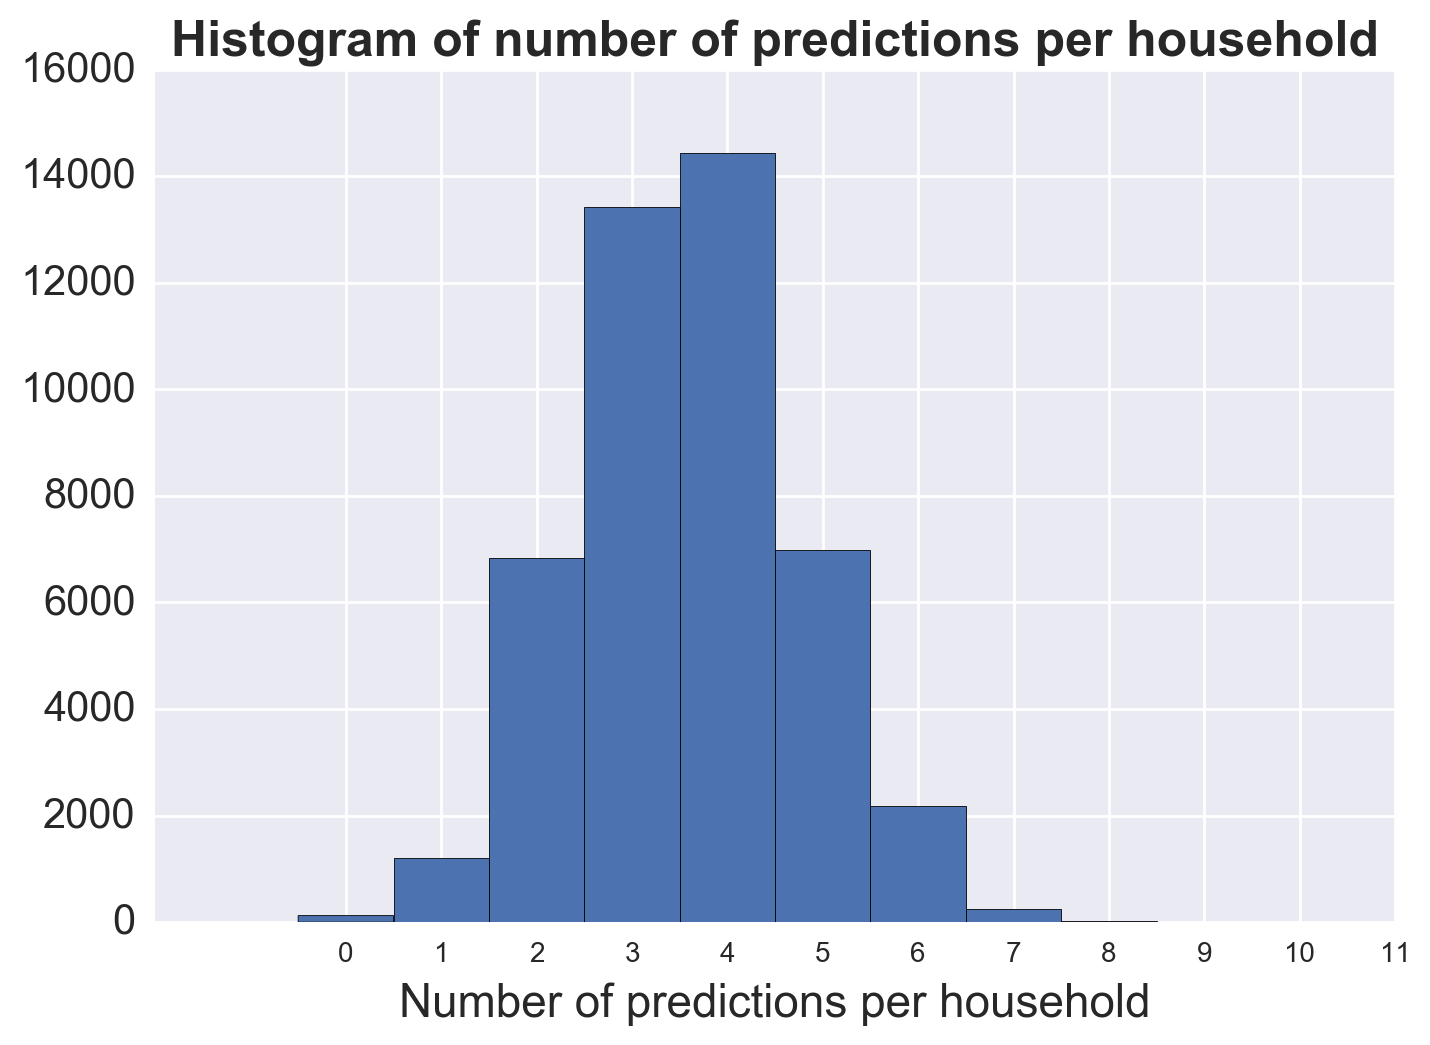
\includegraphics[width=.9\linewidth]{predictionHistogram2.png}
%  %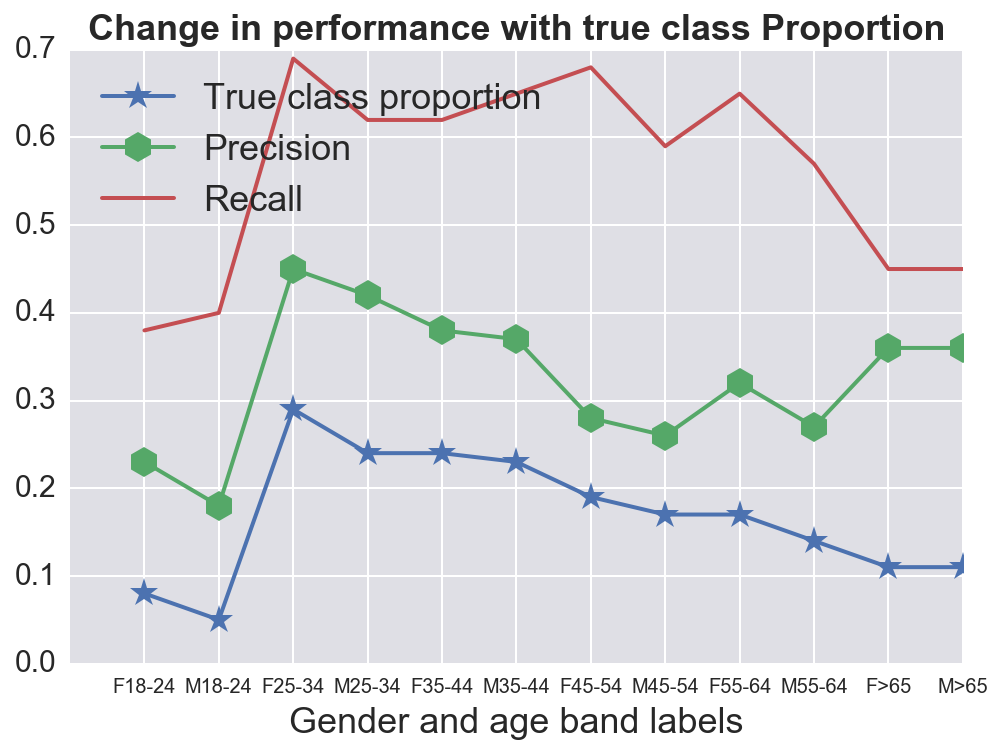
\includegraphics[width=.45\linewidth]{br_allLabels2.png}
%  \caption{Distribution of number of persons per household predicted by Binary Relevance.}
%  \label{fig:histogram-br}
%\end{figure}
\subsection{Jointly discovering age and gender composition}
In this experiment our goal is to jointly predict the age and gender of each member in a household. We used K-Multi-household data (essentially 2-household) for training and evaluation. From the 220K households in K-Multi-household, we used 70\% for training, 10\% for validation (to tune the threshold for each label) and 20\% for evaluation. For each data point a 12-dim vector (6 age band $\times$ 2 gender) is used as target.  Binary relevance (BR) has been implemented with 12 independent XGBoost binary classifiers optimizing logistic loss. The performance numbers are reported in Table \ref{table:performance-age-gender}. We see that exact match accuracy of binary relevance is very low. This is due to over-prediction by BR. While the ground truth has 2 labels for almost all households, binary relevance predicts 4 members in 32\% household and 3 members in 30\% household as shown in the histogram in Figure \ref{fig:histogram-br} (left). This may be due to the missing label issue in the dataset. When we select the threshold to predict exactly two members in a household, the exact match accuracy improves (referred as BR-Max-2) by 1312 bps on K-Multi-household data. We also see that the performance of BR is correlated with the class proportion. Figure \ref{fig:histogram-br} (right) demonstrates that the precision and recall, which are more effective measures under class imbalance setting, are proportional to the true class proportion.

To exploit the dependencies between the labels, we trained conditional Bernoulli mixture model (CBM) with gradient boosted decision trees as individual classifiers. Clearly CBM outperforms Binary relevance and its variants by at least 566 bps. We see that 99\% of the predictions of CBM are 2-household. CBM detects the correlation that dominant number of households are two persons of same age band and opposite genders and almost every time its predictions lie inside those compositions as shown in Figure \ref{fig:histogram-cbm}. We see CBM to be mostly confused among the nearby age bands, e.g., \{Female with age $>$ 65 and Male with age $>$ 65\} is mostly confused with \{Female with age 55-65 and Male with age 55-65\} . We also evaluated the trained binary relevance and CBM model on MLBLR-survey data and observe similar behavior as with K-Multi-household data.
%\begin{figure}
%  \centering
%  %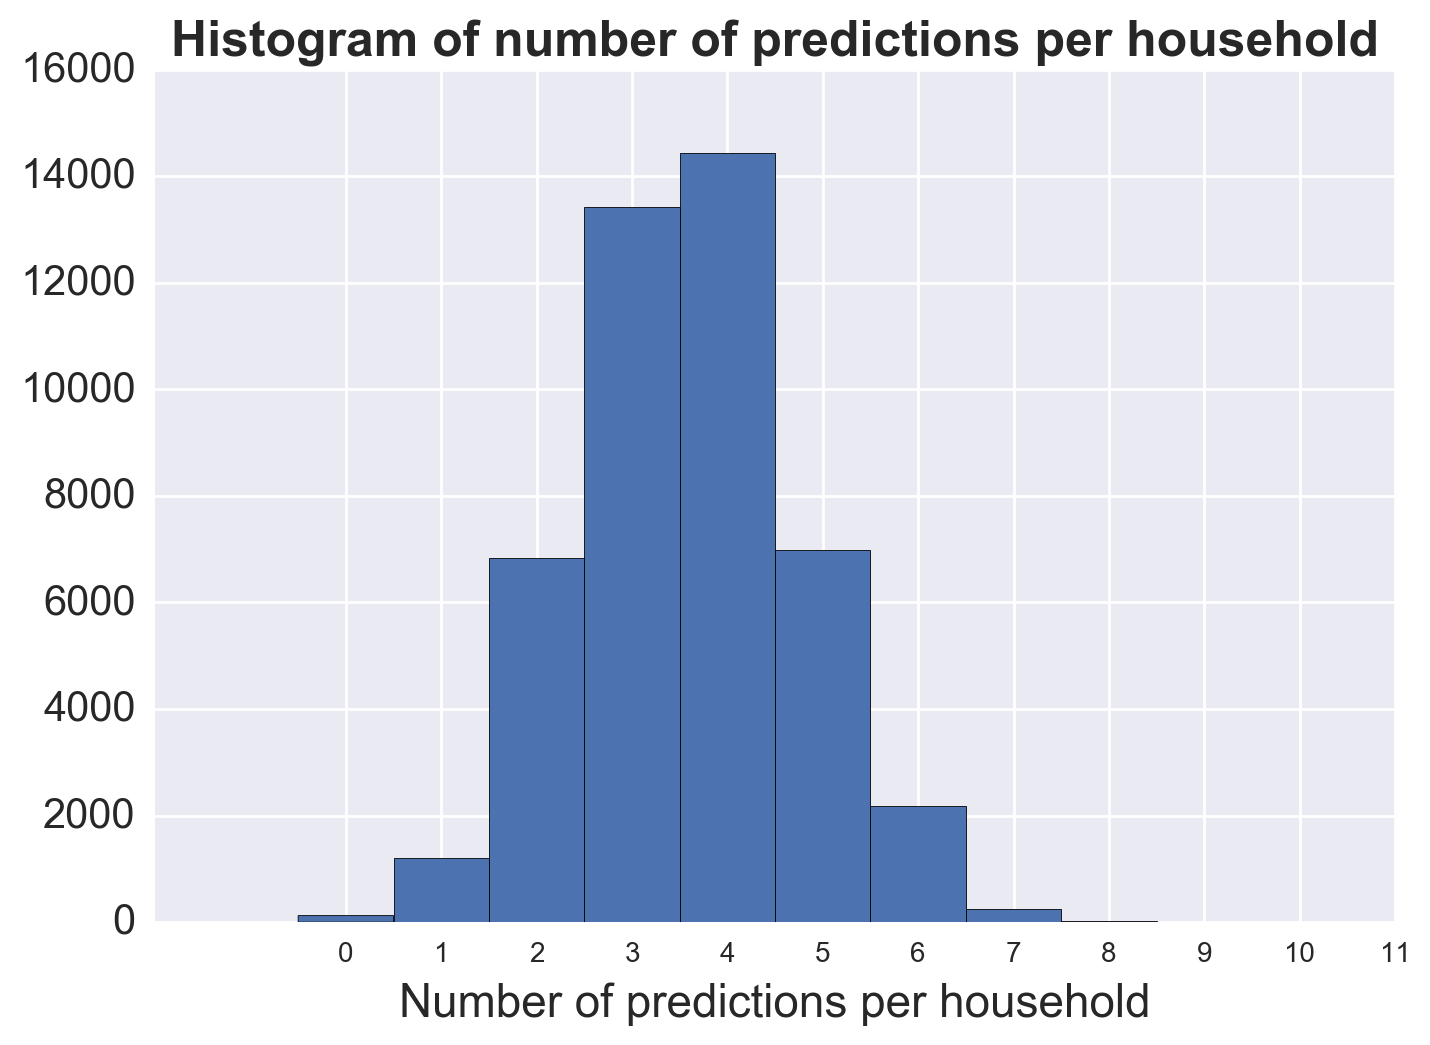
\includegraphics[width=.45\linewidth]{predictionHistogram2.png}
%  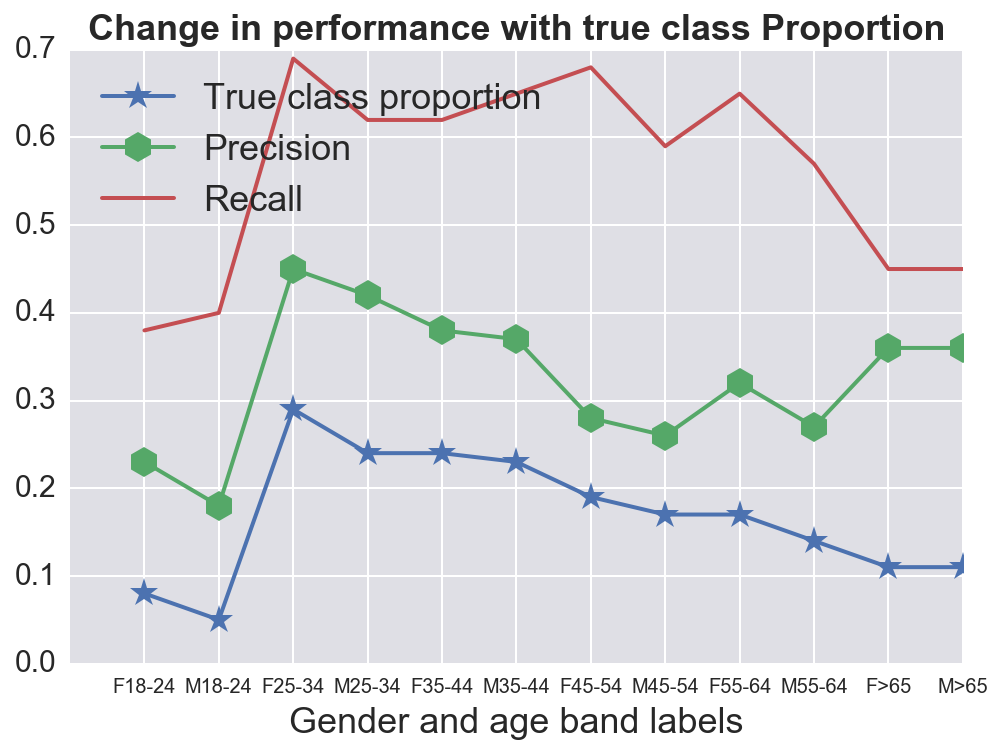
\includegraphics[width=.9\linewidth]{br_allLabels2.png}
%  \caption{Label wise precision and recall with increasing threshold.}
%  \label{fig:br2}
%\end{figure}
%\vfill
%
%The top features learnt by XGBoost BR is presented in figure \ref{fig:topfeatures-XGBoost} where we see some intuitive title features to be mapped to the right age bands, e.g., words like ``pregnancy", ``ovulation" are mapped to [female, age 25-35] and the GL lawn and garden to be mapped to [male, Age 55-65].


\subsection{Discovering age composition}
To investigate the ability of the algorithms in identifying the age composition of households, we experiment with the 6 age groups as labels. We train the binary relevance and XGBoost-multiclass on a random sample of Experian and evaluate the trained models on Kindle household, K-multi-household and MLBLR-survey data. As CBM needs a truly multilabel data, we train it on a random 70\% of K-Multi-household data.   The performance numbers are reported in Table \ref{table:performance-age}. We see that CBM outperforms binary relevance in most of the cases and Multiclass XGBoost outperforms both CBM and binary relevance. This is because, after transforming the 12 labels to 6 labels, 42\% of the accounts in K-Multi-household data contain only one age band which makes the training difficult for truly multilabel algorithms like CBM.
%while CBM is trained on a multi-labeled data with missing labels, multiclass XGBoost is trained on a multiclass dataset. The test datasets are mostly single household and the multiclass XGBoost is able to cover sizable amount of single households. 
Again, instead of using gradient boosted decision trees as individual classifiers of CBM, if we use XGBoost the performance of CBM may improve further.
%mainly due to the missing labels in the train and test set for the multilabel algorithms. In contrast the multiclass XGBoost is trained with Experian which is a multiclass dataset. 
%We also see that CBM performs little worse in K-multi-household data. This is because, .  
%
%
\subsection{Experiment with noisy labels}
In this section, we demonstrate the effect of noisy labels in the training set on the performance of XGBoost. 
%We flip the labels of a clean data, to analyze the effects of the flips on the model performance. 
We artificially introduce different levels of label noise into a clean dataset and examine the behavior of XGBoost when trained on the noisy data. 
To obtain a clean dataset we trained XGBoost on Experian and filtered the training set by choosing customers with zero training error. Then we flipped x$\%$ labels of this clean data, trained multiple XGBoost models and computed their accuracy on predicting ICT labels. The plot in Figure \ref{fig:labelNoise1} demonstrates the change in performance as we increase x from 0 to 40. This conveys that XGBoost is arguably robust to the label noise, e.g., corrupting 40\% labels takes down the performance by only 570 bps (from 49.4 to 43.7). A simple extrapolation of this observation, suggest that if Experian is 30\% noisy, fixing Experian may improve the performance by $\sim$ 380 bps. 

Now the question we ask is, can we fix Experian by examining the training loss? To see this we use the setup of \cite{pmlr-v70-koh17a} as described in the following. The goal is to identify the flipped data points based on the training loss. 
%We identify a subset of the training set that will represent the noisy dataset. We call this subset as candidate set.
 \begin{figure}
\captionsetup{font=small}
\setlength{\belowcaptionskip}{-10pt}
  \centering
  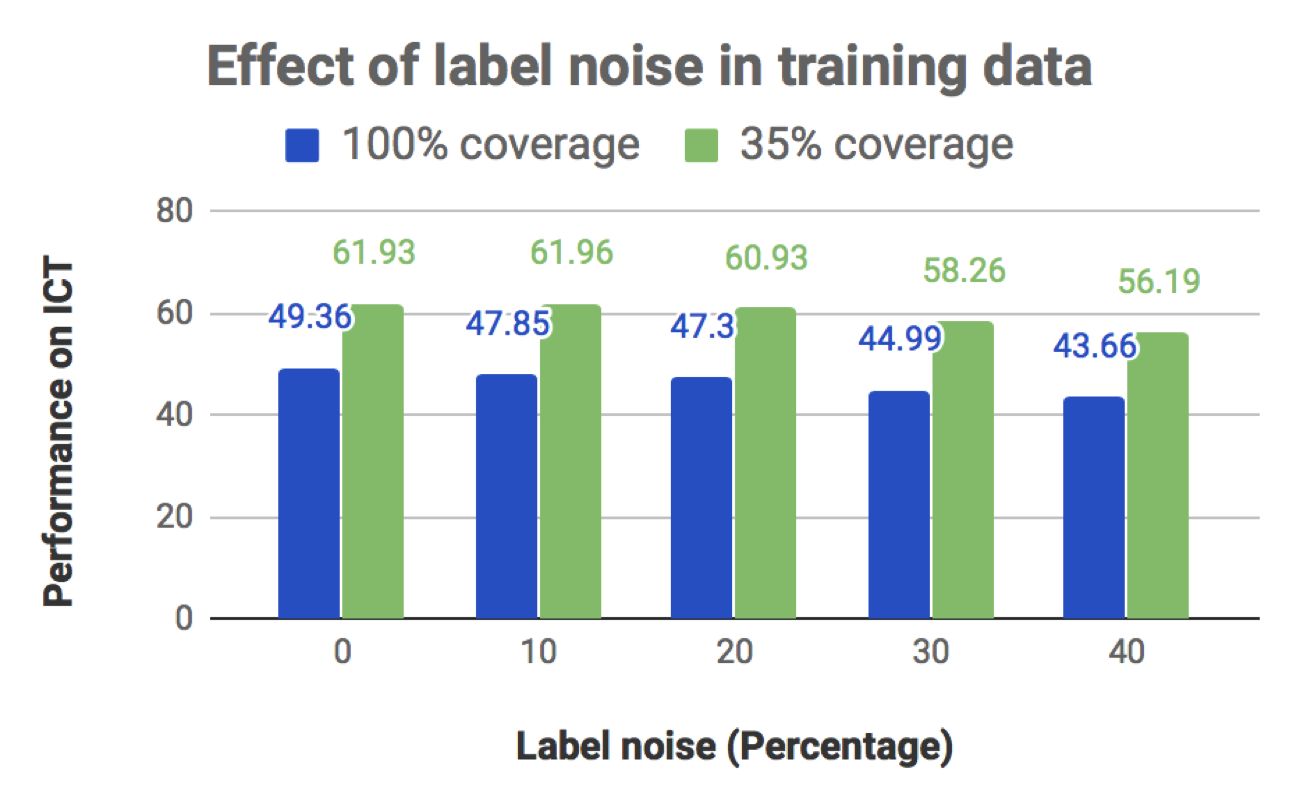
\includegraphics[width=0.92\linewidth]{Plots/labelNoise1.png}
  %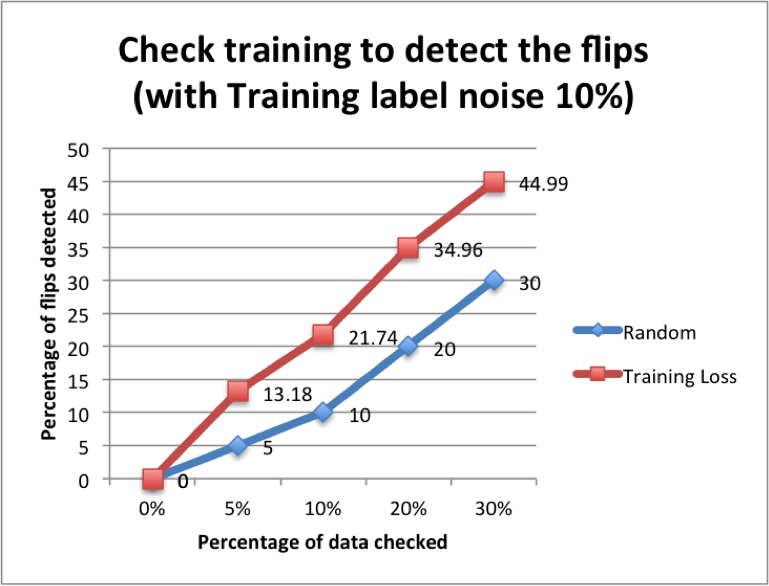
\includegraphics[width=.4\linewidth]{Plots/labelNoise2.png}
  \caption{Effect of training label noise on performance.}
  \label{fig:labelNoise1}
\end{figure}
Same as earlier, we obtained a clean dataset by selecting customers with zero training error and flipped 10\% of its labels to form a corrupted training set. Then we trained a XGBoost model on this corrupted training set and considered data points with high training loss as our candidate set for the corrupted labels. 
%The training loss is computed as: (1-probability of the data point being mapped to the training labels).
%
The plot in Figure \ref{fig:labelNoise2} demonstrates the size of the candidate set as a fraction of the training set versus the fraction of corrupted labels covered in the candidate set. We see top 5\% of the training set (as per train loss) covers almost 13\% of the flips. We compare this with the ``Random approach", where data points are selected randomly instead of considering training loss. 
\begin{figure}
\captionsetup{font=small}
\setlength{\belowcaptionskip}{-5pt}
  \centering
  %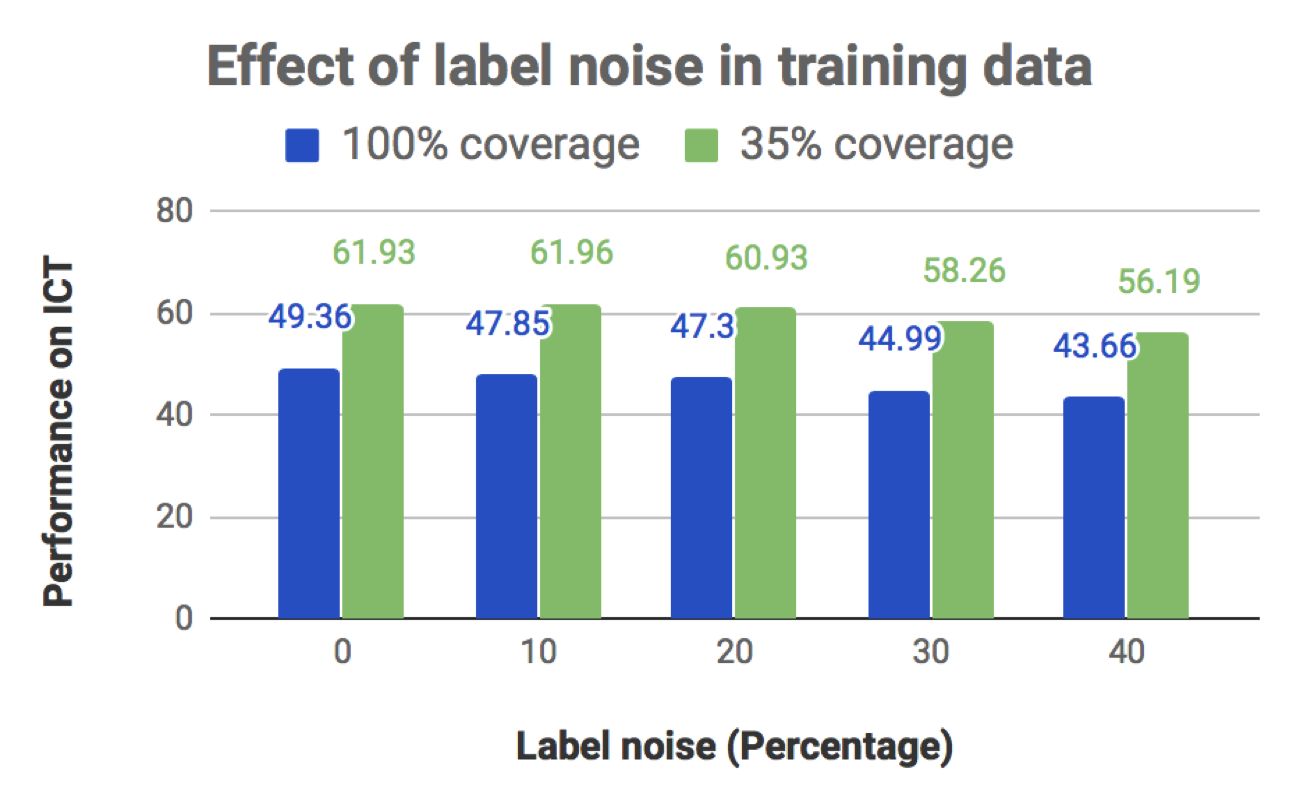
\includegraphics[width=0.4\linewidth]{Plots/labelNoise1.png}
  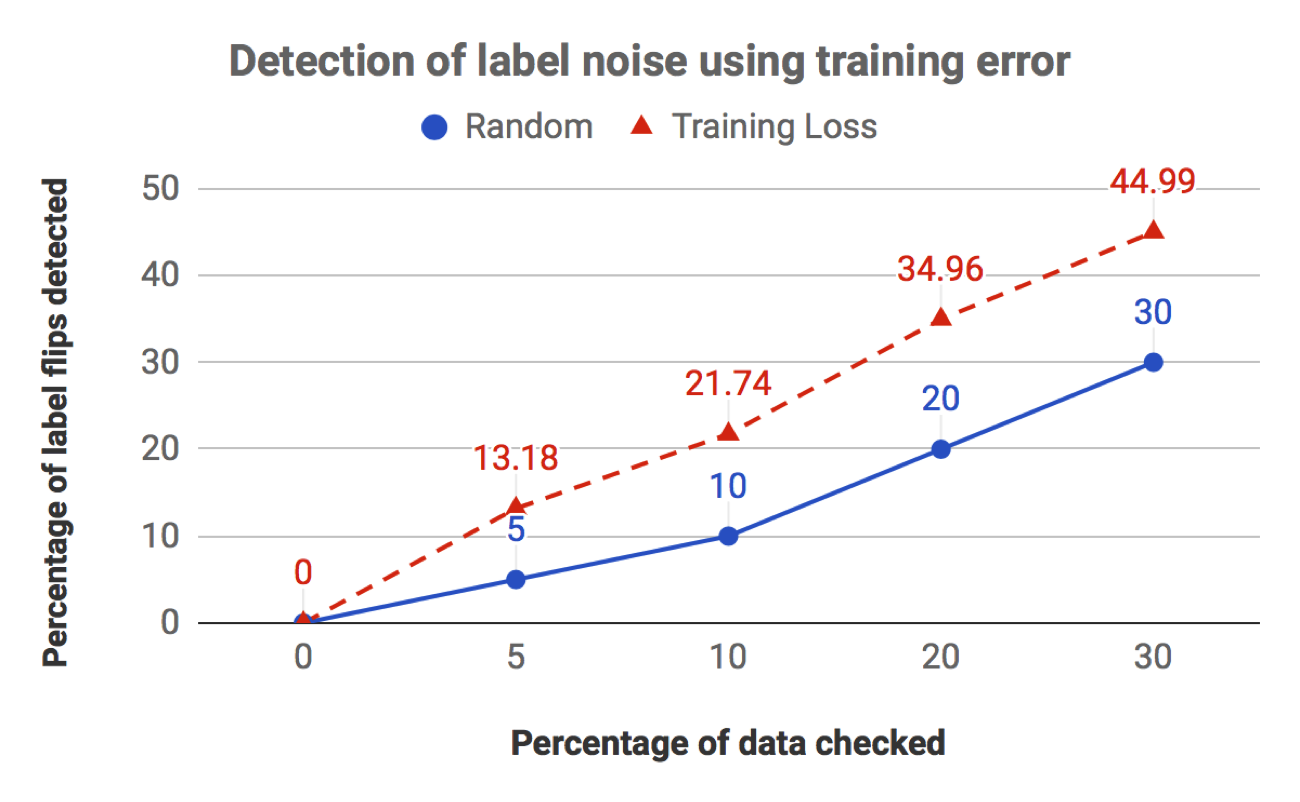
\includegraphics[width=.92\linewidth]{Plots/labelNoise3.png}
  \caption{Identifying label flips by examining training error}
  \label{fig:labelNoise2}
\end{figure}
Clearly, considering the training loss to detect label flips is better than selecting randomly. However the precision is still low, e.g., precision at top 5\% candidate set is 
 %$\frac{0.1318 * \#flippedLabels}{0.05 * \#trainingPoints}$ = 26.2\%  
26.2\% with recall 13.18\%. This suggests that training loss based approaches to identify the label flips are not that effective and better approaches are required to identify the label corruptions. 
%We leave this as a future work. 
\begin{table}[]
\small
\captionsetup{font=small}
\setlength{\belowcaptionskip}{-15pt}
\centering
\begin{tabular}{|c|c|c|}
\hline
\textbf{Match Levels}     & \textbf{\begin{tabular}[c]{@{}c@{}}Accuracy \\ @100\% Cov.\end{tabular}} & \textbf{\begin{tabular}[c]{@{}c@{}}Accuracy \\ @35\% Cov.\end{tabular}} \\ \hline
All levels                & 50.5                                                                            & 65.6                                                                           \\ \hline
Match Level \textless= 11 & 50.6                                                                         & 65.2                                                                        \\ \hline
Match Level \textless= 3  & 51.5                                                                         & 66.1                                                                        \\ \hline
\end{tabular}
\caption{Performance on ICT at different match levels.}
\label{tab:match-experiment}
\end{table}
\vfill
%
\textbf{Experiment with Match criteria}\\
The Experian data that we use to train our models has been obtained by joining age information provided by Experian (a third party organization) with Amazon customers. The join happens over many attributes, e.g., Email, zip code, first name, etc. and can use any combination of these features as well. The join criteria has been classified into 17 match levels. An example of a match level could be $\{$email, first name, address$\}$.  Each customer in Experian has been joined with Amazon customer base using a join criteria from these 17 match levels. We conjecture that the label error in Experian is partly induced by this matching and labels of customers matched with strong match levels is of higher quality than that matched with weaker ones. 
%
To observe this empirically, we train models on 1.5M customers with match level limited to $<=3$, $<=11$ and $<=17$ with lower index indicating stronger criteria. We evaluate the models on the ICT data to see their ability to predict account holder's age group and present the results in Table ~\ref{tab:match-experiment}.  We see our conjecture to be valid and performance of the model improves with stronger match levels, e.g., by restricting the match level to $<=$ 3 the multiclass accuracy at 100\% coverage has improved by 100 bps. We note here that 
%\vspace{-5mm}
the performance of the model improves further by increasing the number of training customers, e.g., we see a boost of 220 bps in the accuracy at 35\% coverage (to 67.8\%) by increasing the training customers to 3.4M . This suggests that the model should ideally be trained on more number of customers with strong match levels to obtain high performance.
\begin{figure}[]
  \captionsetup{font=small}
  \centering
    \centering\includegraphics[width=0.45\textwidth]{importantASINs/error0.png}
  \caption{Explanation of prediction error: Account with ground truth age $>65$ is predicted to be in age group 35-44. We see the purchases are most likely from a person of 35-44 for kids.}
  \label{fig:error_analysis}
\end{figure}
\begin{figure*}[ht]
  \captionsetup{font=small}
%  \setlength{\belowcaptionskip}{-15pt}
  \centering
  \begin{subfigure}[b]{0.5\linewidth}
    \caption{\textbf{Age : 18-24}}
    \centering\includegraphics[width=0.95\textwidth]{importantASINs/age1_v1.png}
  \end{subfigure}%
  \begin{subfigure}[b]{0.5\linewidth}
    \caption{\textbf{Age : 25-34}}
    \centering\includegraphics[width=0.95\textwidth]{importantASINs/age2_v2.png}
  \end{subfigure}
\\
    \begin{subfigure}[b]{0.5\linewidth}
    \caption{\textbf{Age : 35-44}}
    \centering\includegraphics[width=0.95\textwidth]{importantASINs/age3_v2.png}
  \end{subfigure}%
  \begin{subfigure}[b]{0.5\linewidth}
    \caption{\textbf{Age : 45-54}}
    \centering\includegraphics[width=0.95\textwidth]{importantASINs/age4_v1.png}
  \end{subfigure}
\\
  \begin{subfigure}[b]{0.5\linewidth}
    \caption{\textbf{Age : 55-64}}
    \centering\includegraphics[width=0.95\textwidth]{importantASINs/age5_v1.png}
  \end{subfigure}%
  \begin{subfigure}[b]{0.5\linewidth}
    \caption{\textbf{Age group: Above 65}}
    \centering\includegraphics[width=0.95\textwidth]{importantASINs/age6_v1.png}
  \end{subfigure}
  \caption{Top important ASINs for each age group learnt by XGBoost.}
  \label{fig:important_asins}
\end{figure*}
%
\begin{table}[]
\small
\setlength{\belowcaptionskip}{-15pt}
  \captionsetup{font=small}
\centering
\begin{tabular}{|c|c|c|c|}
\hline
\textbf{Rank} & \textbf{\begin{tabular}[c]{@{}c@{}}Accuracy\\ @100\% Cov.\end{tabular}} & \textbf{\begin{tabular}[c]{@{}c@{}}Accuracy\\ @35\% Cov.\end{tabular}} & \textbf{\begin{tabular}[c]{@{}c@{}}\% of variance\\ captured\end{tabular}} \\ \hline
100           & 43.3                                                                    & 56.3                                                                   & 33.2                                                                       \\ \hline
200           & 44.2                                                                    & 57.7                                                                   & 37.6                                                                       \\ \hline
400           & 44.5                                                                    & 58.2                                                                   & 44                                                                         \\ \hline
800           & 43.9                                                                    & 56.6                                                                   & 53.6                                                                       \\ \hline
Full rank     & 45.6                                                                    & 58.3                                                                   & 100                                                                         \\ \hline
\end{tabular}
\caption{Performance on ICT by model trained on low rank approximations (SVD) of the data.}
\label{tab:svd-experiment}
\end{table}
%
%\vspace*{\fill}
%\\\\
\subsection{Removing feature noise using Low rank approximation (SVD)}%\\
In general customers order for different persons in their household and share accounts among friends and relatives. This adds noise in the purchase data while trying to discover the household age composition. In an effort to filter out this noise from the data we experimented with the low-rank approximation of the data. 
%
More specifically we performed singular value decomposition (SVD) on the data matrix $A_{n\times d}$ ($n$ customers with $d$ features each) to obtain $A \approx U_{n\times k}\cdot D_{k \times k} \cdot V_{d \times k}^{T} $. We experimented with different values for the rank ($k$) and considered rows of $U$ to be the low rank approximation of the customer features.  We trained XGBoost multiclass classifiers on 500K customers from Experian data and used the low rank approximations as features. We evaluated our model on ICT data to see the quality of the model on predicting account holder's age band and present the results in Table ~\ref{tab:svd-experiment}. We observe that the performance of the model increases with increase in rank but after rank=$400$ it drops. Also, the variance covered by the approximation at rank 400 is just 44\%. This suggests that, either the data have high amount of noise or the data is too complex to be modeled in a linear framework. To examine further we computed the performance by a model trained on all features with no dimension reduction. As the performance without dimension reduction is close to the performance with features approximated to rank 400, we remark that more than 50\% of the variance in the data is due to noise and XGBoost is providing competitive performance by ignoring this noise.
%
%
\subsection{Explanations of predictions}
%Understanding predictions of a machine learning model is vital to ensure the user's trust on the model. 
In general, users expect some interpretable explanations which can help them to reason and trust the model. 
Here we intend to explain the XGBoost model trained on the account holder's age group, by identifying the ASINs most responsible to make predictions. We compute the importance of each ASIN by the following procedure. For each ASIN, we created a synthetic customer with purchase of only that ASIN and predicted the age band of the synthetic customer. We considered the confidence in prediction as the importance of the respective ASIN. Some of the most important ASINs in each age group is presented in Figure ~\ref{fig:important_asins}. Clearly the identified ASINs are relevant for their respective age groups, e.g., the ASINs under age groups 55-64 and above 65, are relevant to senior citizens. We also see, the age groups between age 25 and age 55, are being identified by ASINs that are most likely for their kids.

To understand the prediction error, we analyze the accounts where the predictions' absolute deviation from the ground truth is greater than 1. We see around 10\% of the accounts fall under this category. After looking into the ASINs purchased by these accounts, we found the ASINs to be relevant for the predicted age group rather than the ground truth. For example, while the ground truth is of age above 65, the model predicted age group 35-44 due to the kid's purchases as shown in Figure ~\ref{fig:error_analysis}. In some other accounts we see the prediction error is due to purchases of ambiguous ASINs, e.g., a book for GRE preparation can map to age group 25-34 or 45-54. In these cases, XGBoost gets confused between the two age bands and arbitrarily predicts one of the age band. 
%We also see the prediction error to be correlated to the number of purchases. Customers with very high or very low purchases are being predicted incorrectly. 
We also see, customers with very low or very high number of purchases to be predicted incorrectly, e.g., customers with 20 (or 8000) purchases in last 5 years. This is mainly due to the lack of signals when number of purchases is low or excessive noise in the signals when number of purchases is high. 
%
\section{Conclusion}
\label{sec:conclusion}
In this work, we presented the problem of identifying household composition with various challenges involved. We discussed various approaches to address the challenges and experimented with clever multilabel classification algorithms including algorithms exploiting label correlation. 
%The experiments to investigate feature and label noise in the data, provide useful insights.
We presented strong insights from our experiments with feature and label noise in the data.
%
We conjecture that a generative model with ability to represent the data in a complex non-linear way can further improve the predictive quality of the model. Also, more intelligent and scalable techniques to detect label noise can help to improve the quality of labels. Exploring more features, e.g., search data, glance views, etc. can help to express more modalities of the problem leading to an opportunity of improvement.


